% Бүлэг 3

\chapter{Системийн зохиомж}
\label{Chapter3}

%-------------------------------------------------------------------------------
\section{Системийн архитектурын зураглал}
Систем нь клиент--сервер загварт суурилсан, гурван үндсэн хэсгээс бүрдэнэ (Зураг~\ref{fig:arch}): вэб апп, гар утасны апп ба нэгдсэн backend API. Хоёр клиент ижил REST API-г HTTPS/JSON-оор ашигладаг тул бизнесийн дүрэм нэг газар (сервер дээр) хэрэгжиж, клиентүүдийн хооронд зөрөхгүй~\cite{fowler,martin}.

\begin{figure}[H]
\centering
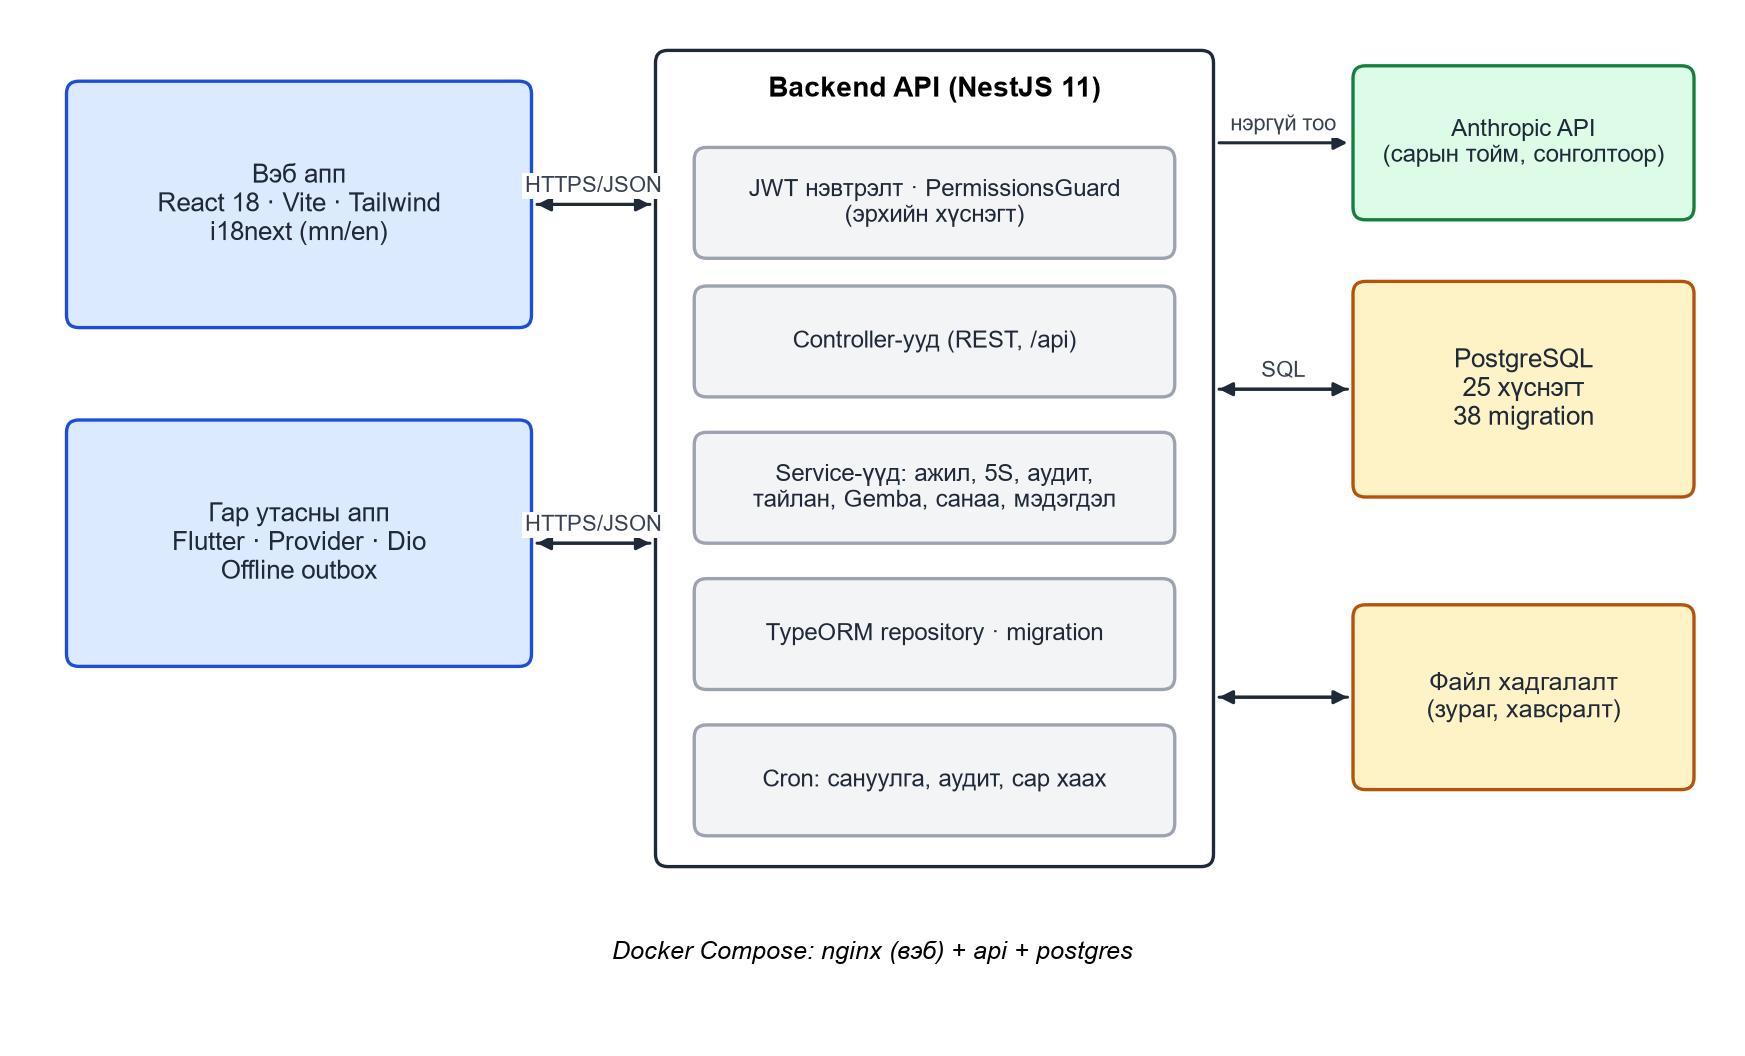
\includegraphics[width=\linewidth]{Figures/architecture.png}
\caption{Системийн архитектур}
\label{fig:arch}
\end{figure}

Backend нь давхаргат бүтэцтэй:
\begin{itemize}
    \item \textbf{Хамгаалалтын давхарга} -- JWT токеныг шалгаж, PermissionsGuard нь маршрут бүрийн шаардсан эрхийг хэрэглэгчийн дүрийн эрхийн хүснэгттэй тулгана. Вэбийн товчлуурыг харуулах эсэх ч мөн энэ хүснэгтээс шийдэгддэг тул клиент, сервер хоёр зөрөхгүй.
    \item \textbf{Controller давхарга} -- HTTP хүсэлтийг хүлээн авч, DTO-оор оролтыг шалгана.
    \item \textbf{Service давхарга} -- бизнесийн дүрэм: ажил, 5S, аудит, тайлан, Gemba, санаа, мэдэгдэл.
    \item \textbf{Өгөгдлийн давхарга} -- TypeORM repository; схемийн өөрчлөлт бүр migration файлаар хийгдэнэ.
    \item \textbf{Цагийн хуваарьт үйлдэл} -- өглөөний сануулга, аудитын хуваарь, сар хаах.
\end{itemize}

%-------------------------------------------------------------------------------
\section{Байршуулалтын диаграмм}
Систем Docker Compose-оор нэг Linux серверт байршина (Зураг~\ref{fig:deploy}). admin-web контейнер (nginx) вэб аппын статик файлыг түгээж, \texttt{/api} хүсэлтийг backend рүү дамжуулна; гар утасны апп API-д HTTPS-ээр шууд хандана. Өгөгдлийн сан болон хавсралт файлууд тусдаа volume-д хадгалагдах тул контейнерийг шинэчлэхэд өгөгдөл алдагдахгүй. Нөөц хуулбар (backup), хяналт (prometheus, grafana), кэш (redis) нь шаардлагатай үед идэвхжүүлэх сонголттой үйлчилгээ юм. Өгөгдлийн сангийн нөөцөөс гадна хавсралтын volume-г тусад нь нөөцлөх шаардлагатай.

\begin{figure}[H]
\centering
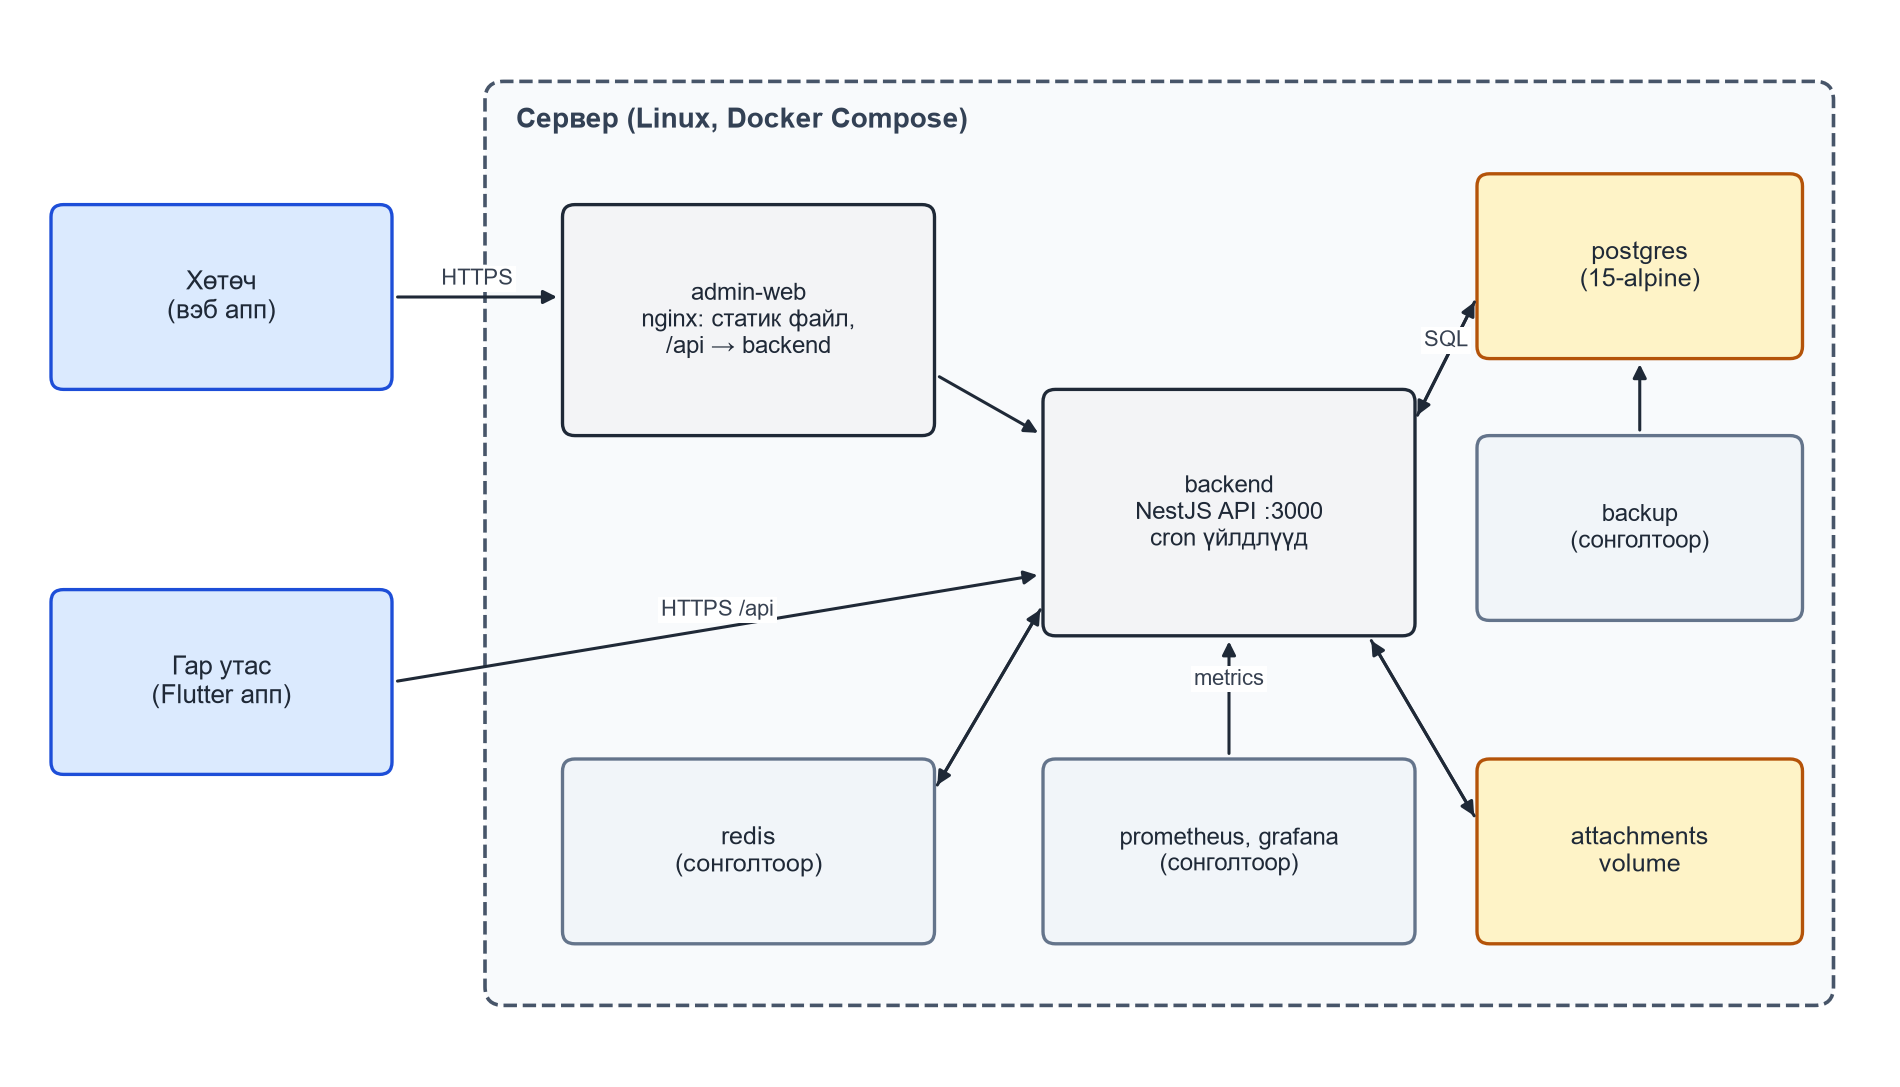
\includegraphics[width=\linewidth]{Figures/deployment.png}
\caption{Байршуулалтын диаграмм}
\label{fig:deploy}
\end{figure}

%-------------------------------------------------------------------------------
\section{Зохиомжийн шатны класс диаграмм}
Зураг~\ref{fig:classD}-д backend-ийн гол классууд ба тэдгээрийн хамаарлыг харуулав. Controller нь guard-аар хамгаалагдаж, service-ийг дуудна; service нь repository-оор дамжин өгөгдлийн сантай ажиллаж, мэдэгдлийн service-ээр хэрэглэгчид мэдэгдэнэ.

\begin{figure}[H]
\centering
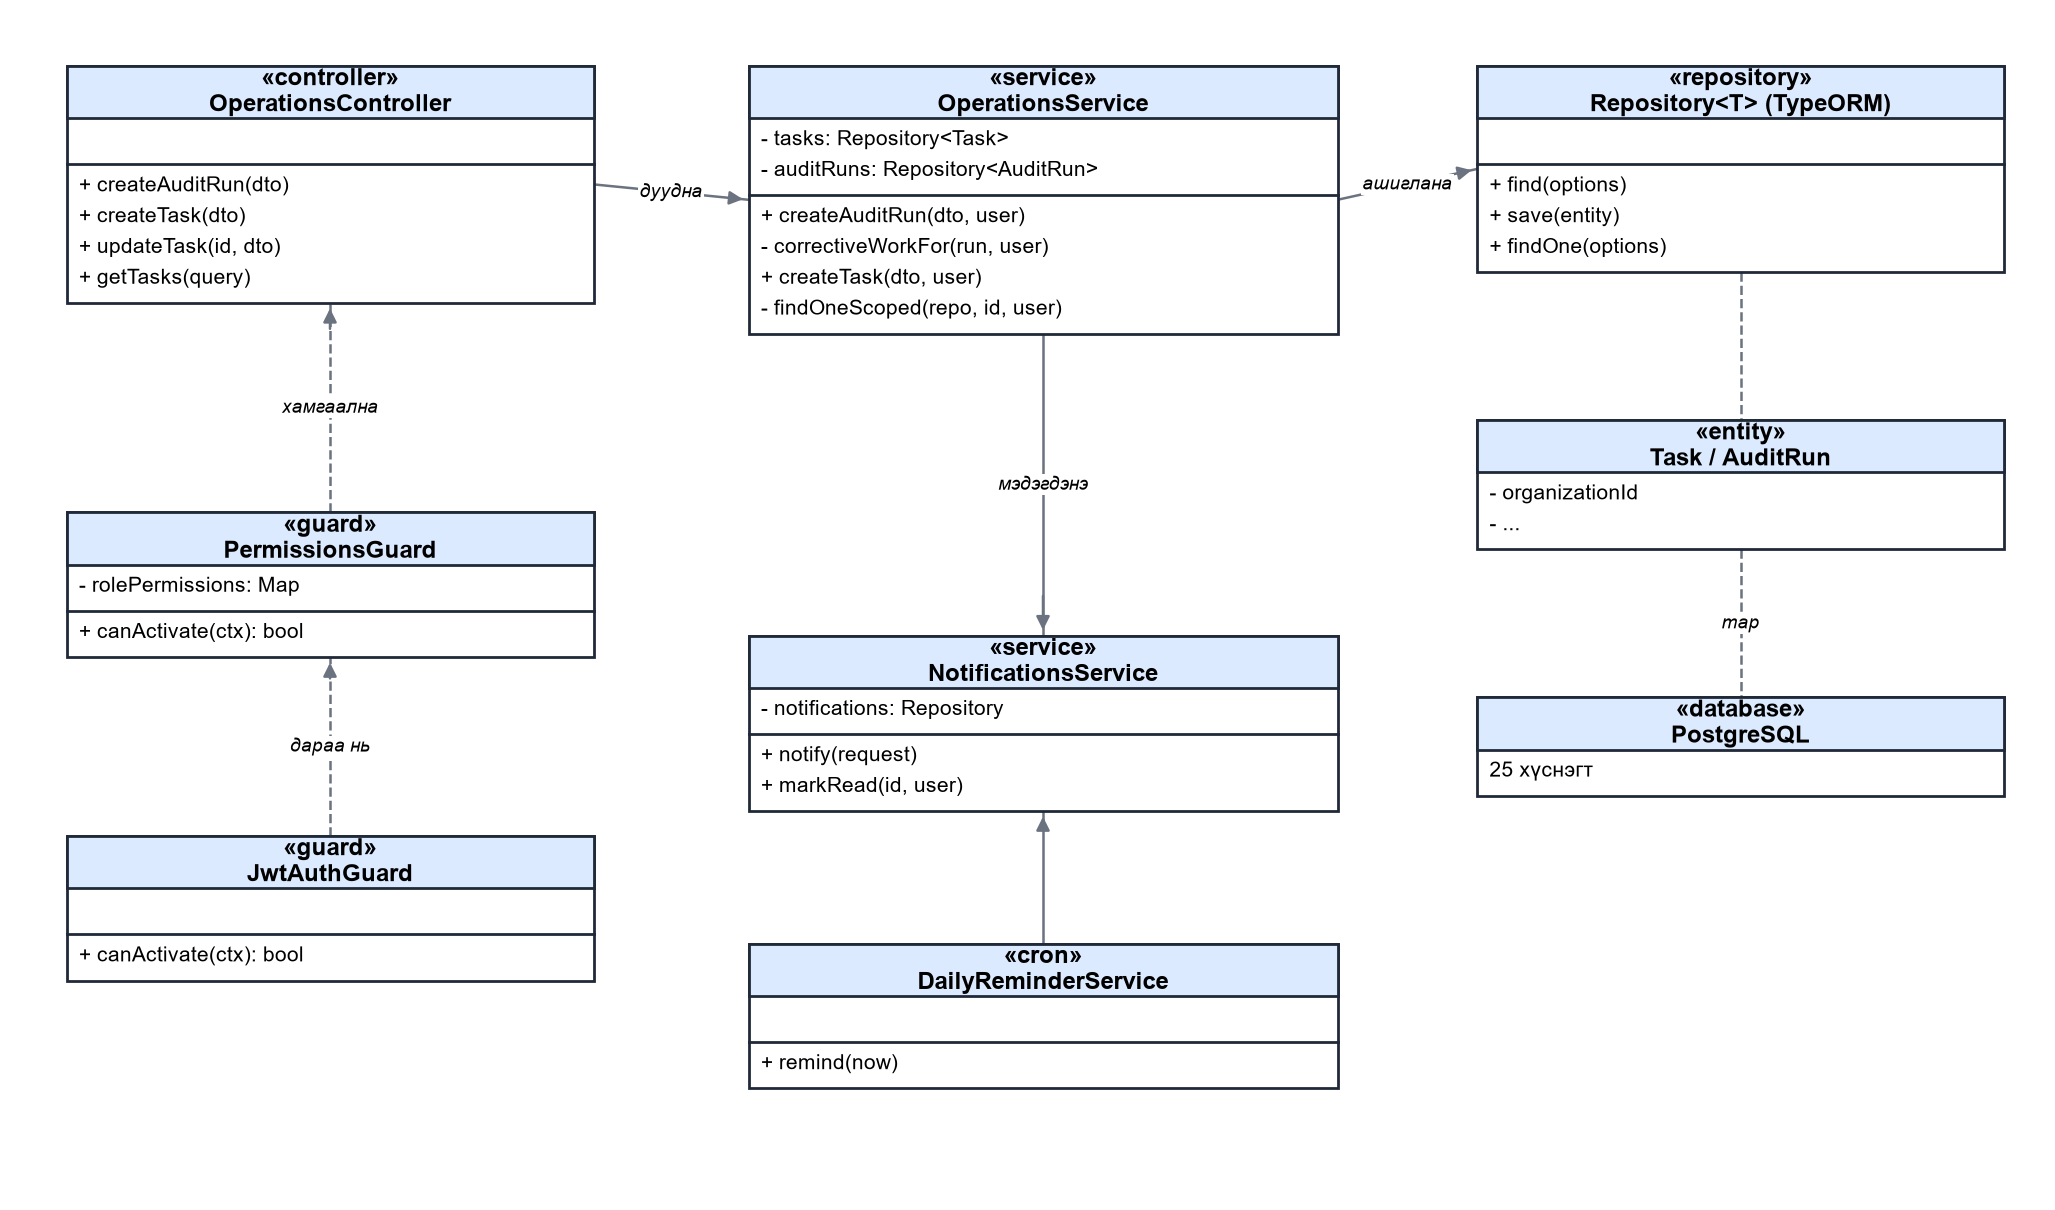
\includegraphics[width=\linewidth]{Figures/class_design.png}
\caption{Зохиомжийн класс диаграмм}
\label{fig:classD}
\end{figure}

%-------------------------------------------------------------------------------
\section{Зохиомжийн шатны дарааллын диаграмм}
Зураг~\ref{fig:seqAudit}-д гар утаснаас 5S аудит хийх, оноо босгоос доош бол засах ажил үүсгэх үйл явцыг харуулав.

\begin{figure}[H]
\centering
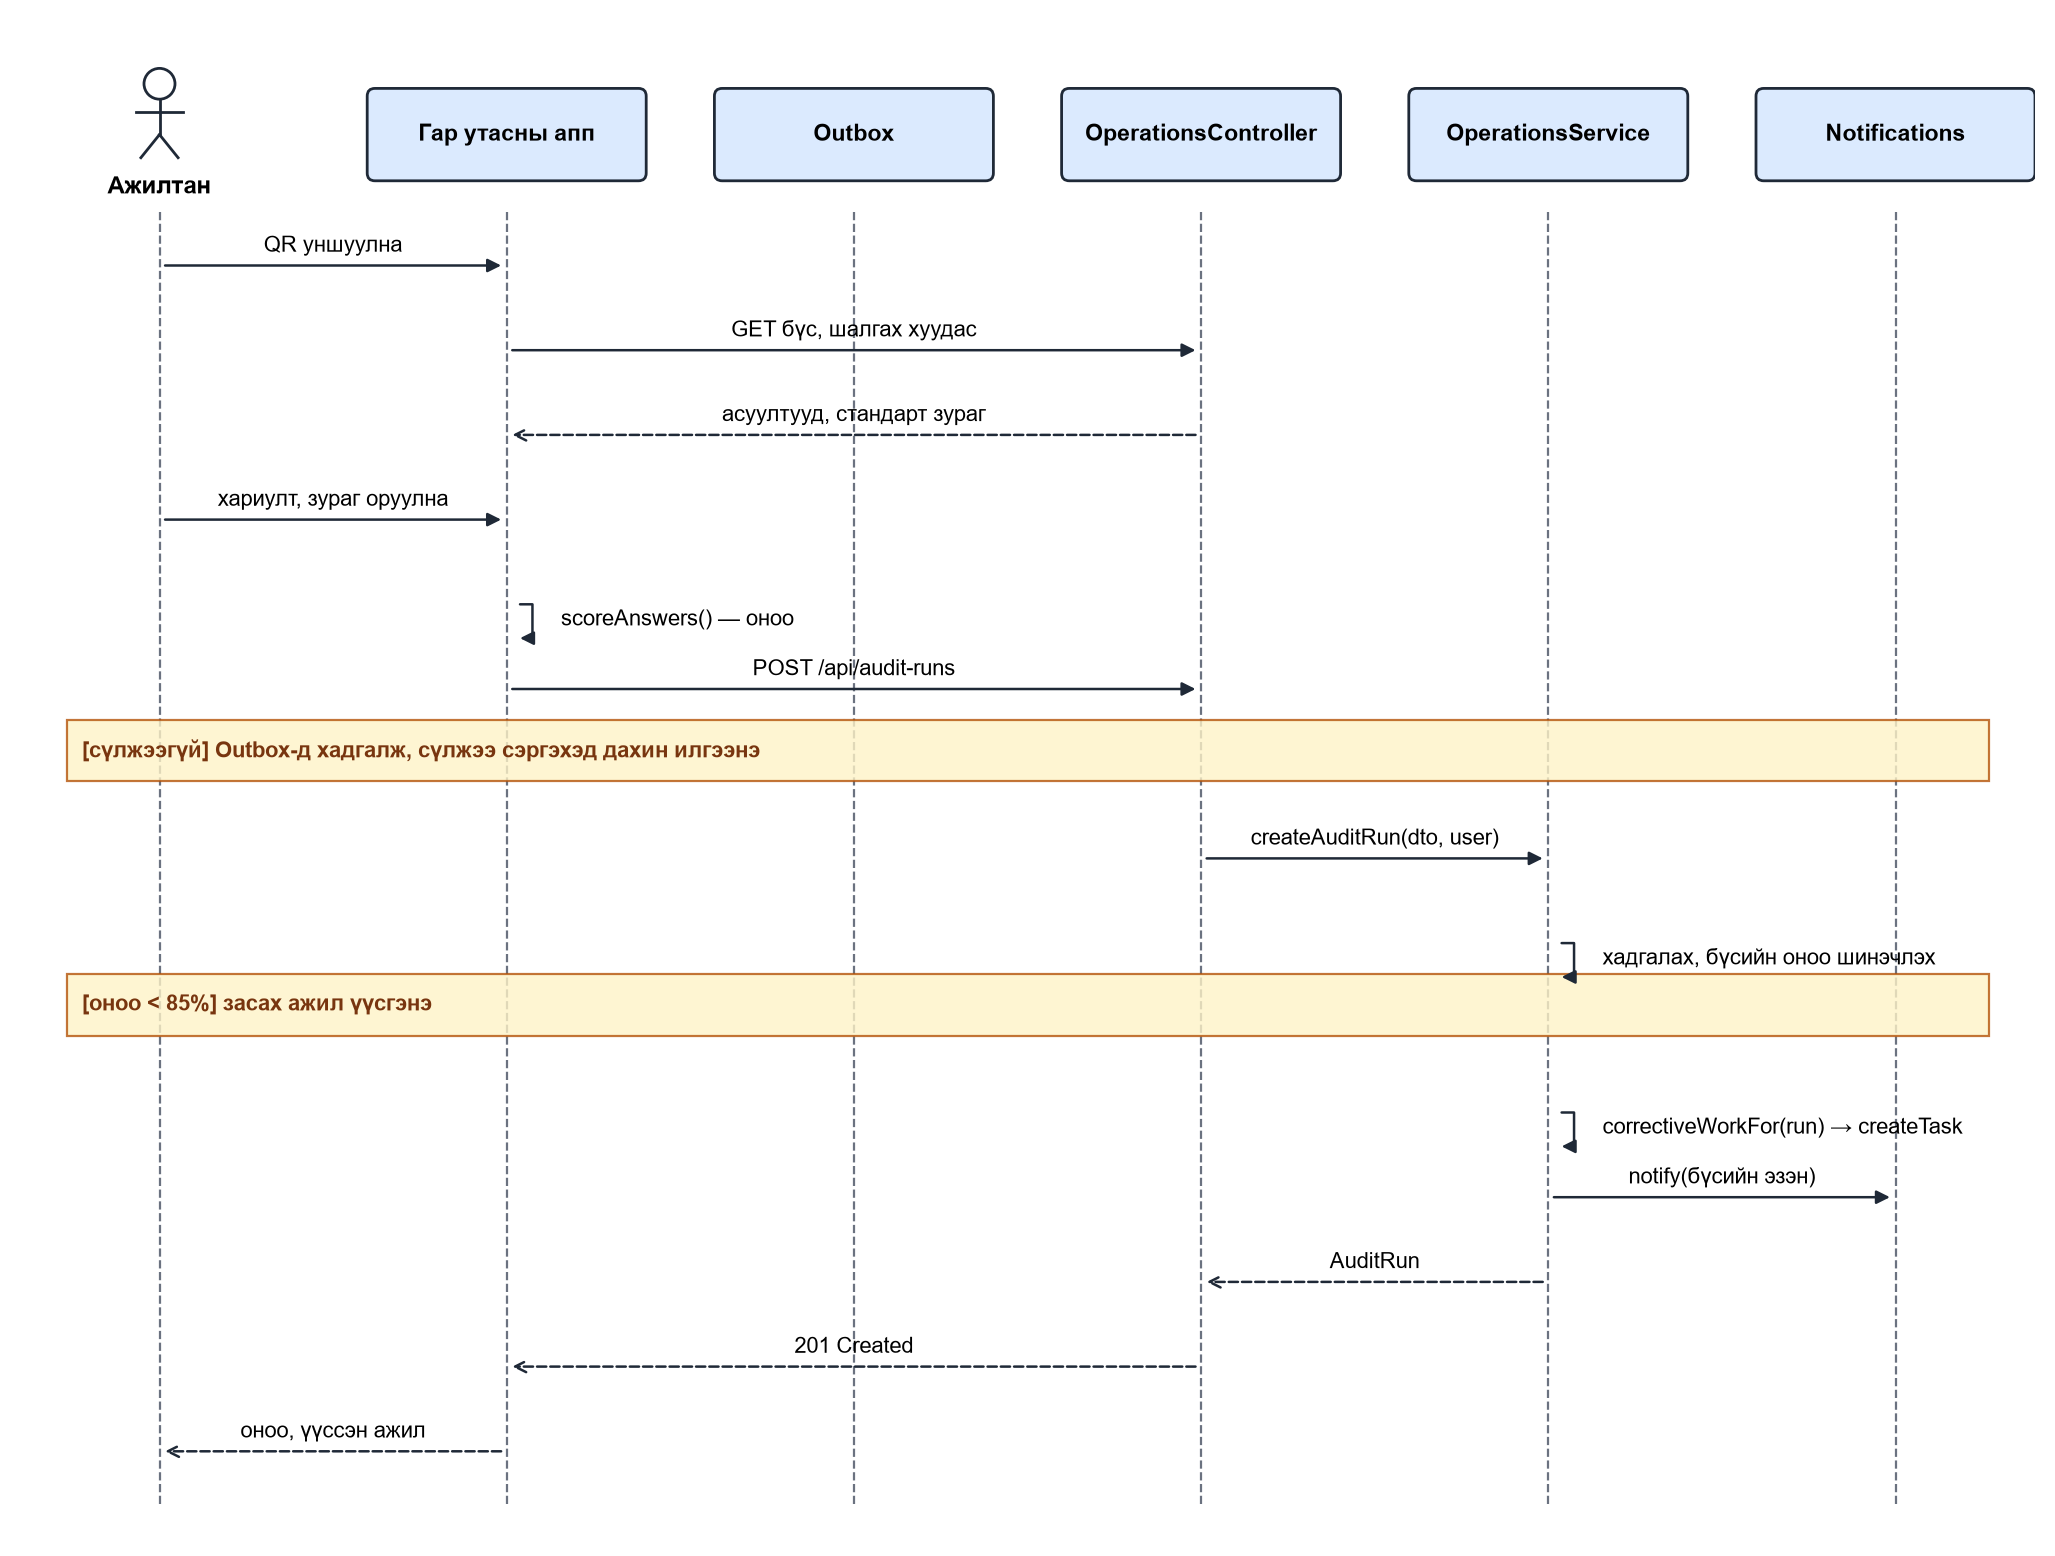
\includegraphics[width=\linewidth]{Figures/seq_audit.png}
\caption{5S аудит хийх зохиомжийн дарааллын диаграмм}
\label{fig:seqAudit}
\end{figure}

Зураг~\ref{fig:seqClose}-д сарын тайланг автоматаар хаах, Зураг~\ref{fig:seqGemba}-д Gemba явалт бүртгэж дараагийн алхмуудыг ажил болгох үйл явцыг харуулав.

\begin{figure}[H]
\centering
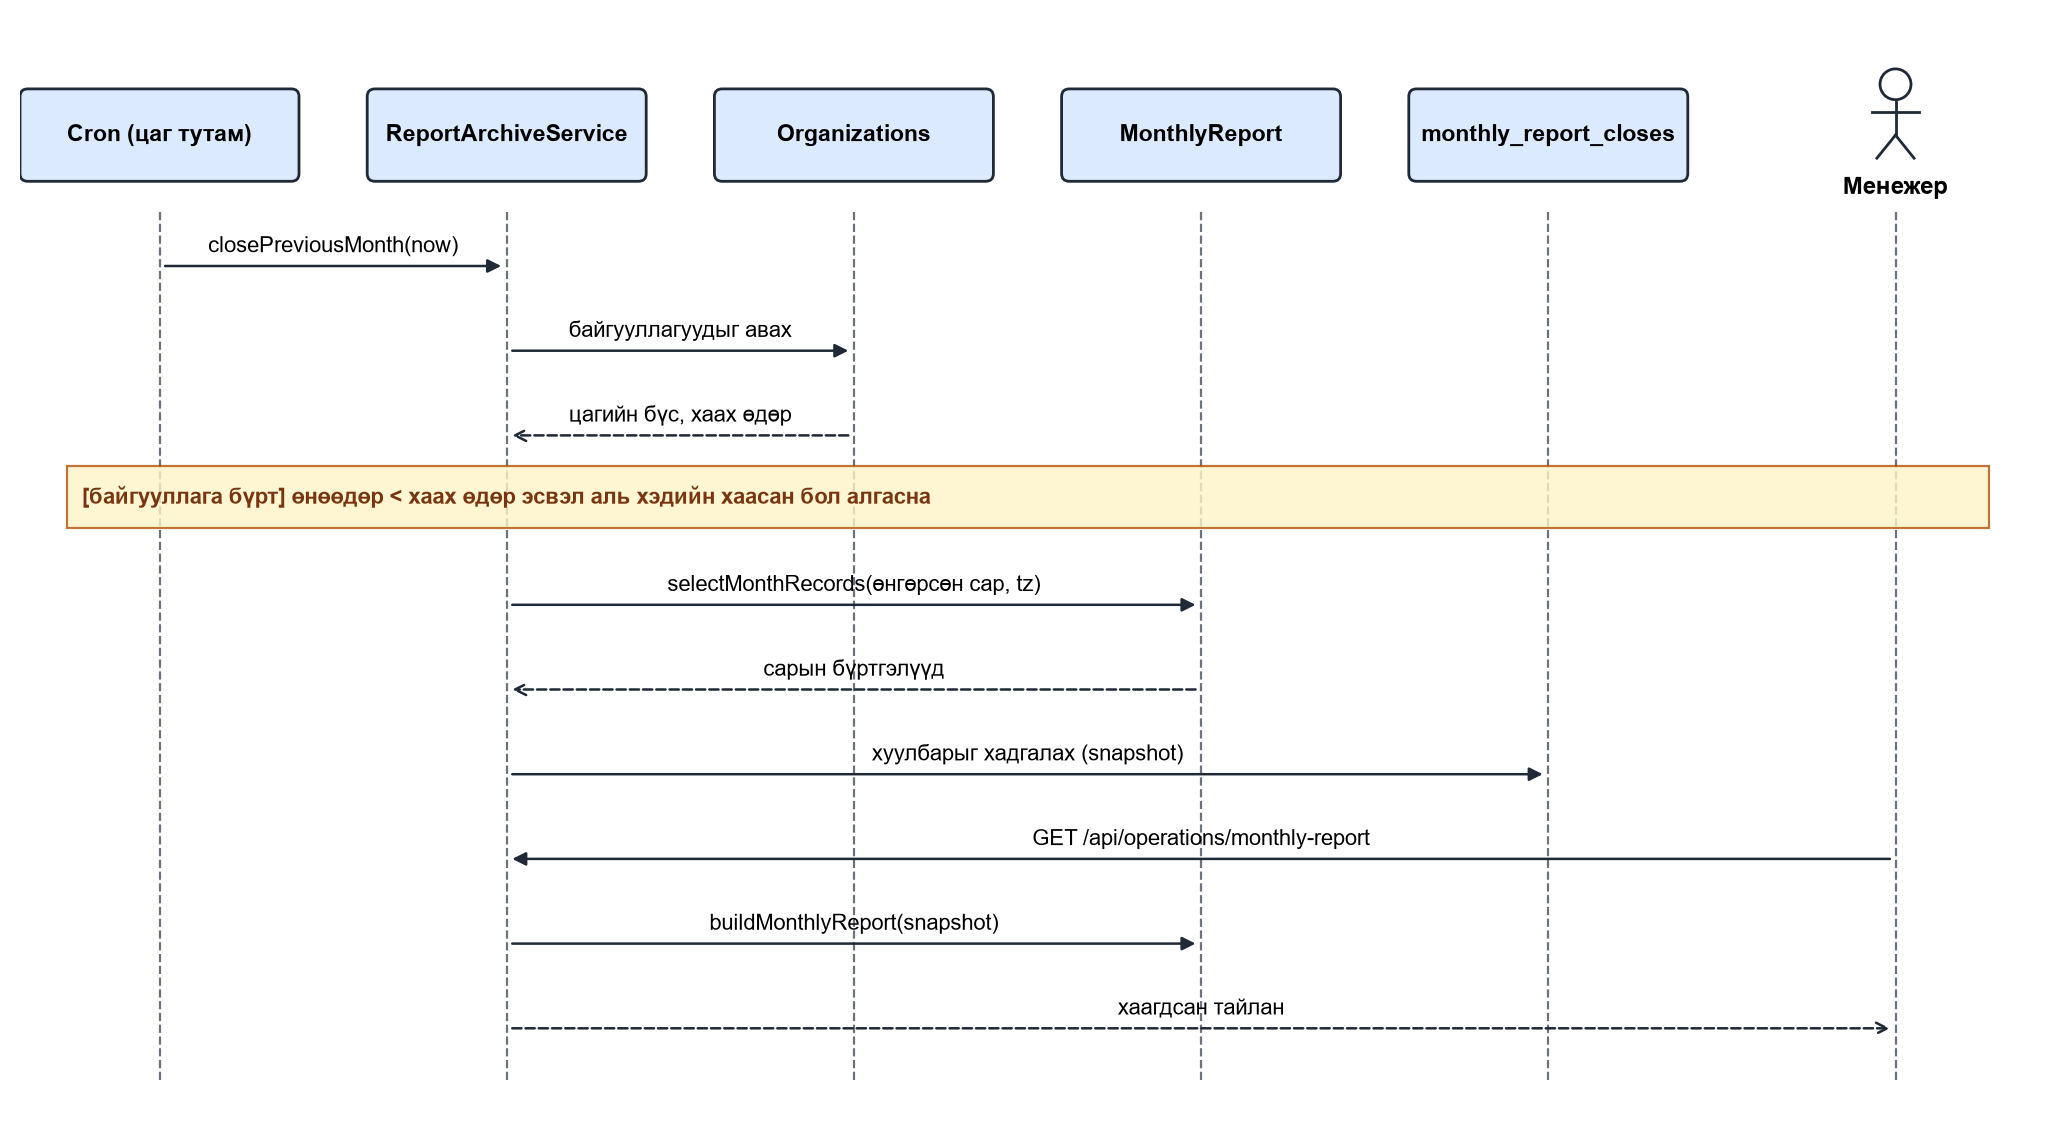
\includegraphics[width=\linewidth]{Figures/seq_close.png}
\caption{Сарын тайлан хаах зохиомжийн дарааллын диаграмм}
\label{fig:seqClose}
\end{figure}

\begin{figure}[H]
\centering
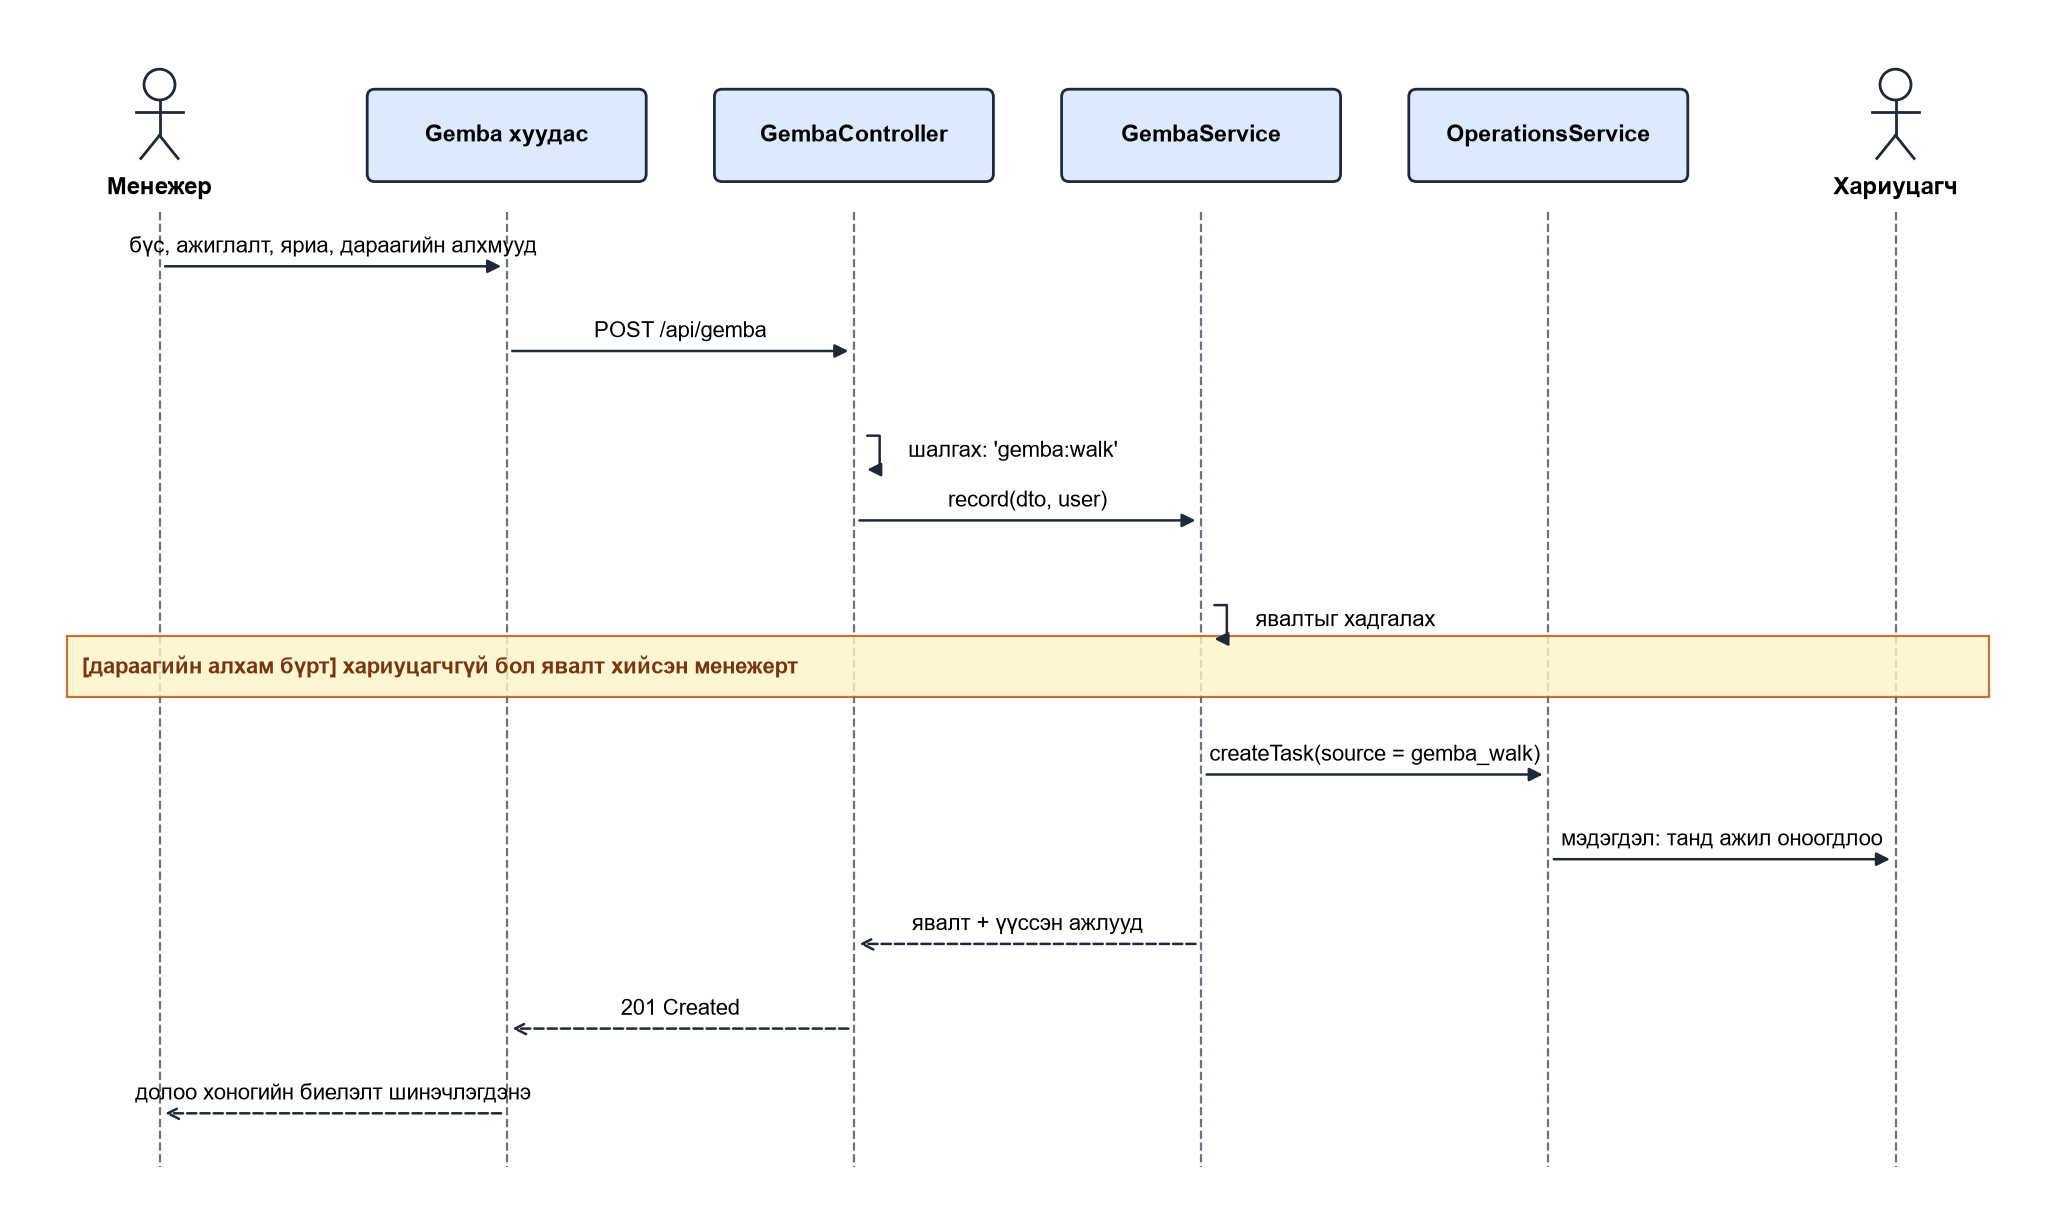
\includegraphics[width=\linewidth]{Figures/seq_gemba.png}
\caption{Gemba явалт бүртгэх зохиомжийн дарааллын диаграмм}
\label{fig:seqGemba}
\end{figure}

%-------------------------------------------------------------------------------
\section{Өгөгдлийн сангийн ерөнхий схем}
Өгөгдлийн сан 25 хүснэгтээс бүрдэх бөгөөд одоогийн схемийг 38 runtime/operations migration-оор байгуулна. Бүх хүснэгт organizationId-аар байгууллагад харьяалагдаж, хүсэлт бүр хэрэглэгчийн байгууллагаар шүүгдэнэ. Зураг~\ref{fig:erd}-д гол хүснэгтүүд ба холбоосыг харуулав.

\begin{figure}[H]
\centering
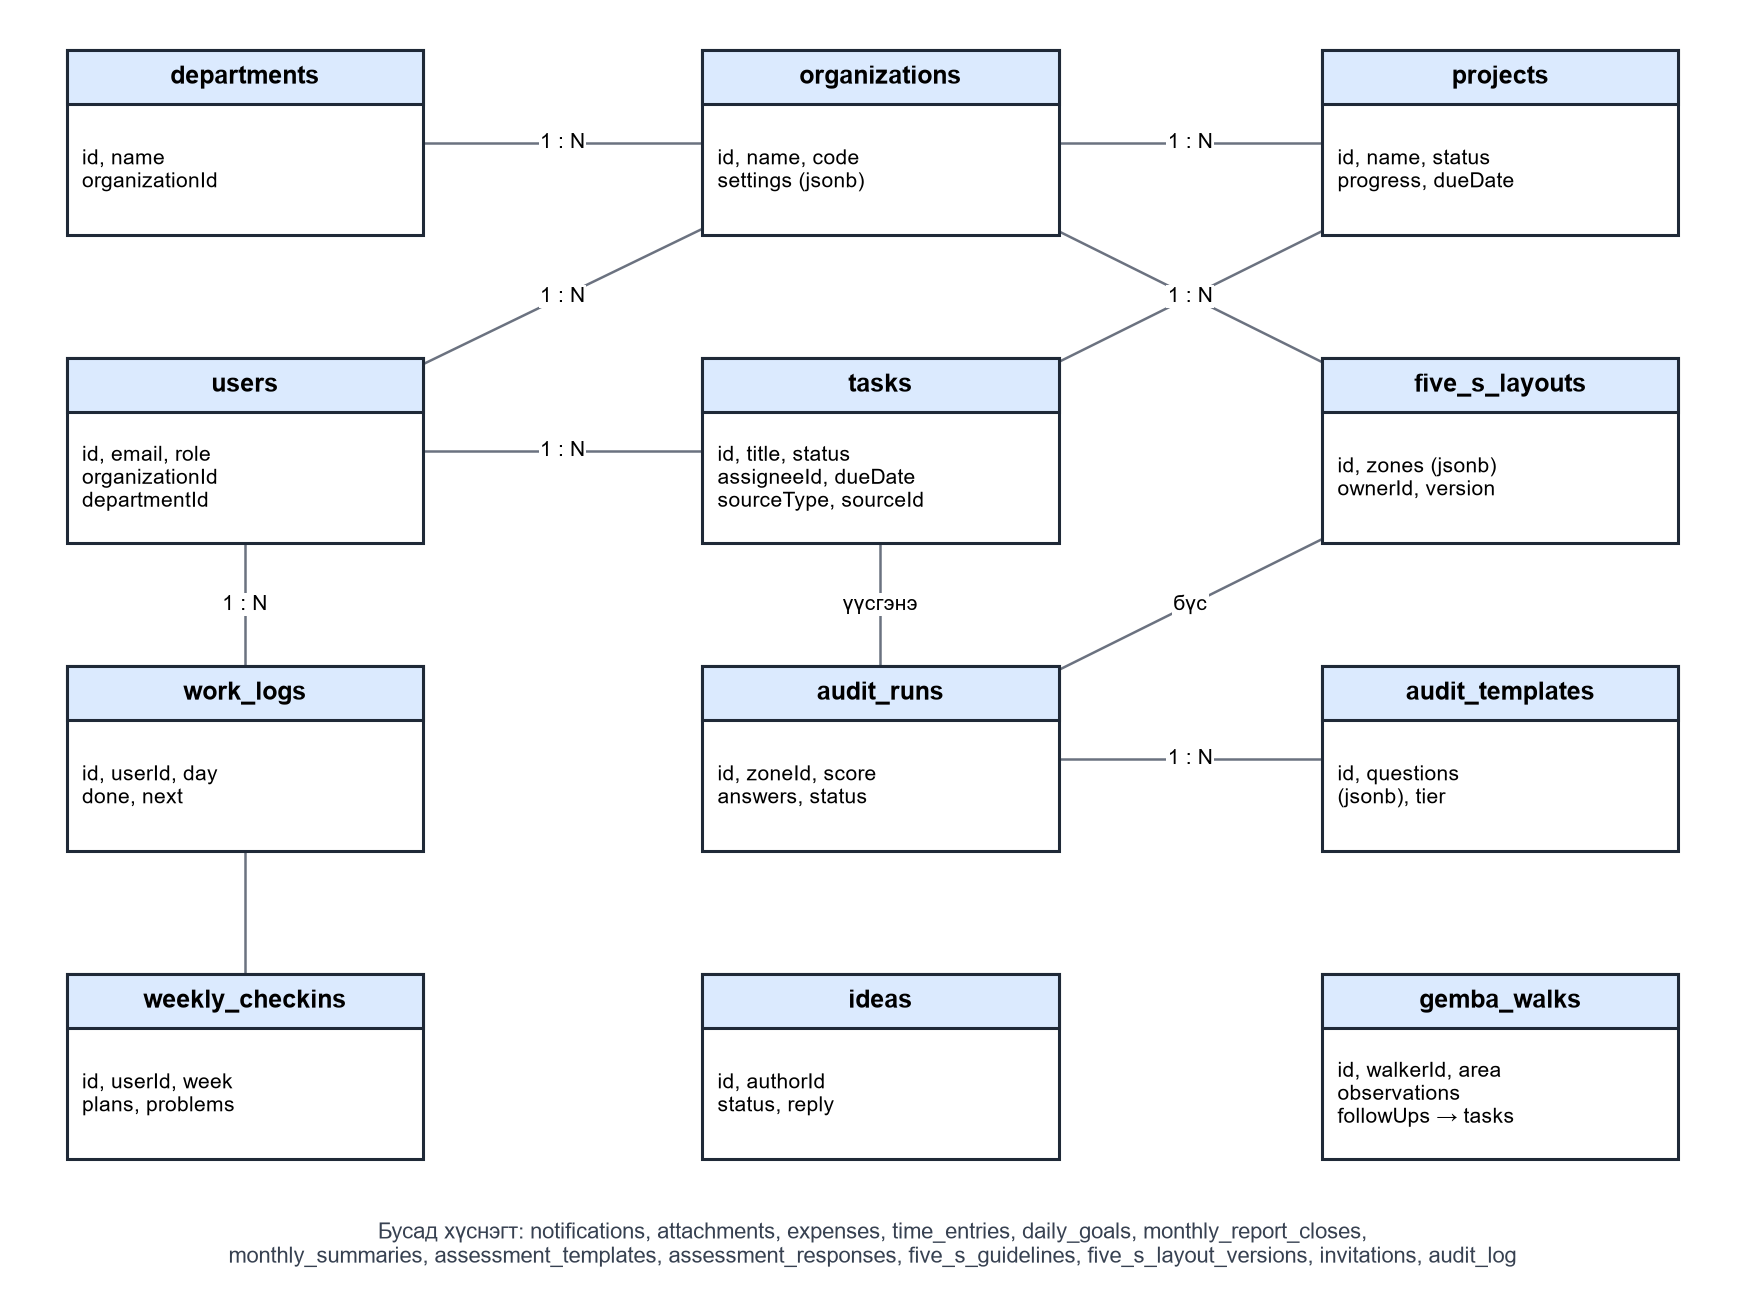
\includegraphics[width=\linewidth]{Figures/er.png}
\caption{Өгөгдлийн сангийн ерөнхий схем}
\label{fig:erd}
\end{figure}

\begin{itemize}
    \item \textbf{tasks} хүснэгт sourceType, sourceId талбараар ажил хаанаас үүссэнийг (аудит, Gemba, санаа, гараар) хадгална. Ингэснээр нэг эх сурвалжаас ажил давхар үүсэхээс сэргийлж, тайланд гарал үүслээр ангилна.
    \item \textbf{five\_s\_layouts} хүснэгт талбайн бүсүүдийг JSONB хэлбэрээр хадгалж, өөрчлөлт бүрийг five\_s\_layout\_versions-д архивлана.
    \item \textbf{monthly\_report\_closes} хүснэгт хаагдсан сарын бүртгэлүүдийн хуулбарыг хадгалж, дараа нь өгөгдөл өөрчлөгдсөн ч тайлан тогтвортой үлдэнэ.
\end{itemize}

%-------------------------------------------------------------------------------
\section{Эрхийн загвар}
Эрхийг дүрд суурилсан хандалтын хяналт (RBAC) аргаар зохион байгуулав. Эрх нь ``нөөц:үйлдэл'' хэлбэртэй (жишээ нь tasks:create, reports:close). Дүр бүрийн эрхийн жагсаалт доод дүрийн жагсаалтыг бүрэн агуулж байхаар хуримтлуулан бичигдсэн тул ``менежер ажилтны бүх эрхтэй'' гэсэн шаардлага бүтцээрээ баталгаажна. Мөн хэрэглэгч зөвхөн өөрөөсөө доод түвшний дүрийг олгох дүрмээр эрх нэмэгдэх замыг хаасан (Эх код~\ref{lst:rbac}).

\begin{lstlisting}[caption={Эрхийн загвар},label={lst:rbac}]
viewer  = [tasks:read, audits:read, reports:read, ideas:read, ...]
user    = viewer  + [tasks:update, audits:create, worklogs:create, ideas:create, ...]
manager = user    + [tasks:create, projects:create, reports:close, gemba:walk, ...]
admin   = manager + [users:update, departments:create, templates:create, ...]

canAccess(user, route) = route.permissions subsetOf permissions(user.role)
canAssign(actor, role) = level(role) < level(actor.role)
\end{lstlisting}

%-------------------------------------------------------------------------------
\section{Алгоритмын зохиомж}
\label{sec:algorithms}

\subsection{Аудитын оноо тооцох ба засах ажил үүсгэх}
Шалгах хуудасны асуулт оноо (0..maxScore, анхдагч 5), тийм/үгүй, текст гэсэн гурван төрөлтэй. Текст хариулт нотолгоо тул оноонд тооцогдохгүй; хариулаагүй онооны асуулт 0 гэж тооцогдоно, учир нь шалгаагүй зүйлийг тэнцсэн гэж үзэх боломжгүй. Оноо нь
\begin{equation}
S = \mathrm{round}\left(\frac{\sum_{q} e_q}{\sum_{q} m_q} \times 100\right)
\end{equation}
энд $e_q$ -- асуултын авсан оноо, $m_q$ -- боломжит дээд оноо. Оноо 85\%-иас доош бол бүсийн хариуцагчид 7 хоногийн хугацаатай засах ажил үүсэх ба 70\%-иас доош бол өндөр ач холбогдолтой болно (Эх код~\ref{lst:audit}).

\begin{lstlisting}[caption={Аудитын оноо ба засах ажил},label={lst:audit}]
function scoreAnswers(template, answers):
    earned = 0; possible = 0
    for q in template.questions:
        if q.type == "score":  possible += q.maxScore or 5; earned += answers[q.id] or 0
        if q.type == "yes_no": possible += 1; earned += (answers[q.id] == "yes") ? 1 : 0
    return possible > 0 ? round(earned / possible * 100) : 0

function correctiveWork(run):
    if run.status == "draft" or run.score >= 85: return null
    zone = zoneOf(run)
    return createTask(title = "5S follow-up: " + zone.name,
                      assignee = zone.owner, due = today + 7 days,
                      priority = run.score < 70 ? high : medium,
                      source = (audit_run, run.id))   // one task per run
\end{lstlisting}

Алгоритмын хугацааны төвөгшил асуултын тоо $n$-ээр $O(n)$. createTask нь (sourceType, sourceId) хосоор давхардлыг шалгадаг тул нэг аудитыг дахин илгээхэд ажил давхардахгүй.

\begin{figure}[H]
\centering
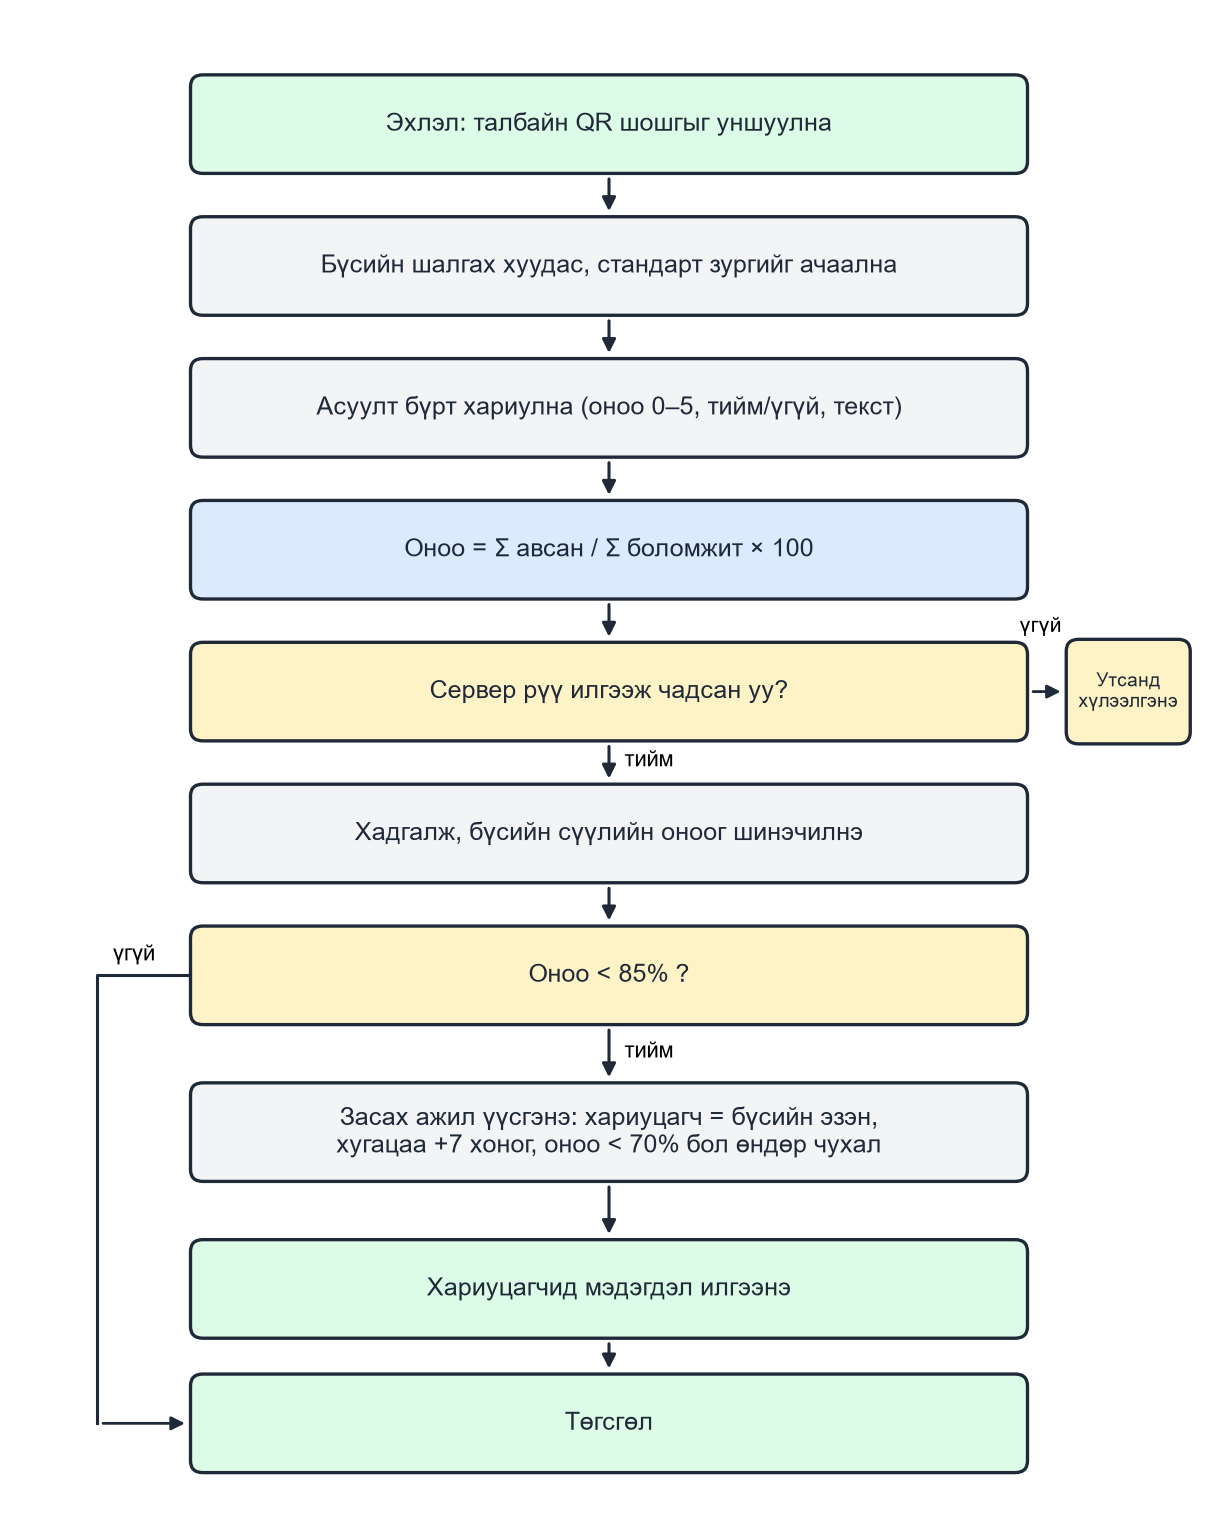
\includegraphics[width=0.62\linewidth]{Figures/audit_flow.png}
\caption{5S аудитын алгоритмын урсгал}
\label{fig:auditflow}
\end{figure}

\subsection{Сүлжээгүй горимын дараалал (outbox)}
5S аудит хийгддэг агуулах, цех, подвал зэрэг газарт сүлжээ тасалдах нь элбэг. Гар утасны апп илгээж чадаагүй бичилтийг хийсэн дарааллаар нь утасны санах ойд хадгалж, сүлжээ сэргэх, апп дахин нээгдэх эсвэл хэрэглэгч ``Одоо илгээх'' дарах үед илгээнэ (Зураг~\ref{fig:outbox}). Гол асуудал нь давхар бүртгэл: хариу ирээгүй хүсэлт серверт хүрсэн байж болно. Иймд зөвхөн серверт огт хүрээгүй нь тодорхой (холболт тогтоогдоогүй) хүсэлтийг дараалалд хийнэ; timeout-ыг дахин илгээхгүй. Дарааллыг илгээх үед сервер 4xx хариугаар татгалзвал тэр бичилтийг хасч хэрэглэгчид мэдэгдэнэ; сервер алдаатай (5xx) эсвэл нэвтрэлт дууссан бол хадгалаад дараа дахин оролдоно.

\begin{figure}[H]
\centering
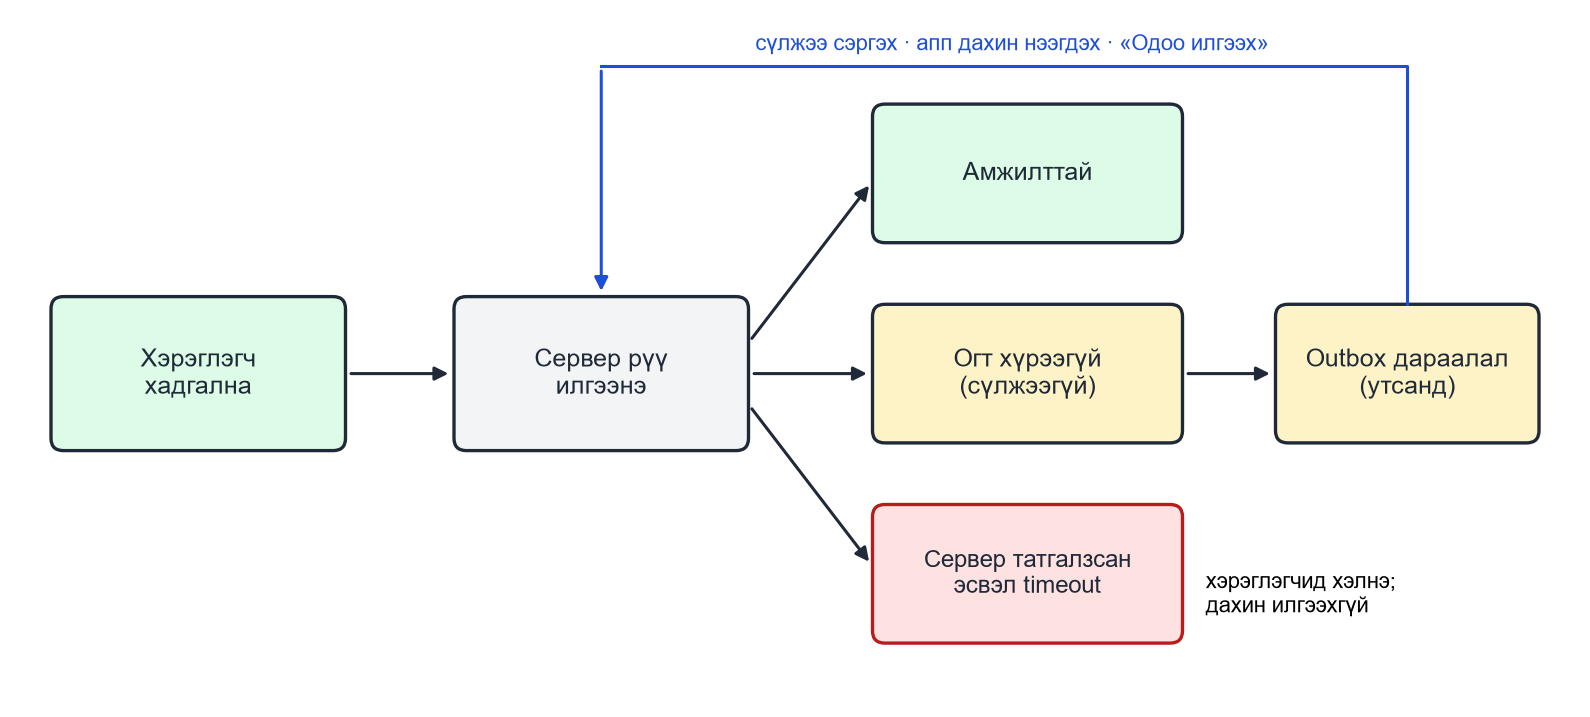
\includegraphics[width=0.9\linewidth]{Figures/outbox.png}
\caption{Сүлжээгүй горимын дарааллын урсгал}
\label{fig:outbox}
\end{figure}

\begin{lstlisting}[caption={Outbox дараалал},label={lst:outbox}]
function save(write):
    try: api.send(write)
    catch error:
        if neverSent(error): outbox.append(write)    // no connection
        else: throw error                           // timeout, 4xx, 5xx

function flush():                                   // network back / app opened
    for write in outbox (in order):
        try: api.send(write); outbox.remove(write)
        catch error:
            if no response or status >= 500 or status == 401: break   // retry later
            outbox.remove(write); refused += 1       // 4xx: final answer
\end{lstlisting}

\subsection{Өдрийн сануулга}
Өглөө бүр ажилтанд тухайн өдөр дуусах болон хоцорсон ажлын жагсаалт, менежерт багийн хоцорсон болон хариуцагчгүй ажлын жагсаалт илгээгдэнэ. Сервер UTC цагаар ажилладаг тул тооцоог байгууллагын цагийн бүсээр хийнэ. Cron цаг тутам ажиллаж, тохируулсан цагаас хойш үдээс өмнөх эхний ажиллалтаар илгээнэ. Мэдэгдлийн эх сурвалж нь тухайн өдөр тул нэг хүнд өдөрт нэгээс илүү сануулга очихгүй (idempotent).

\begin{lstlisting}[caption={Өдрийн сануулга},label={lst:remind}]
every hour:
    for org in organizations:
        tz = org.timeZone; hour = localHour(tz, now)
        if hour < org.reminderHour or hour >= 12: continue
        day = localDate(tz, now)
        for person in org.activeUsers:
            due  = tasks(person) where status not in {done, backlog} and dueDate == day
            late = tasks(person) where status not in {done, backlog} and dueDate <  day
            if (due or late) and not notified(person, source = day):
                notify(person, due, late, source = day)
\end{lstlisting}

\subsection{Сарын тайлан бүрдүүлэх ба хаах}
Сарын тайлан тухайн сарын бүртгэлүүдээс (ажил, аудит, өдрийн болон цагийн бүртгэл, зардал, өдрийн зорилго, үнэлгээ) нэг функцээр тоологдоно. Сар нээлттэй байхад шууд хүснэгтүүдээс, хаагдсаны дараа хадгалсан хуулбараас тоологддог боловч дүрэм нэг тул хоёр үр дүн зөрөхгүй. Биелэлтийн хувь нь ажлын одоогийн төлвөөс бус, хэзээ дууссанаас тооцогдоно:
\begin{equation}
C = \frac{\left|\{t \in P_m : t.\mathrm{completedAt} \le \mathrm{end}(m)\}\right|}{|P_m|}
\end{equation}
энд $P_m$ -- $m$ сард төлөвлөгдсөн ажлын олонлог. Хагас жил, жилийн тайлан хаагдсан сарын тайлангуудын нийлбэр тул батлагдсан сарын тайлантай үргэлж тохирно. Тайлангийн тойм бичвэрийг менежер хүсвэл Claude хэлний загвар ноороглоно~\cite{anthropic}; загвар руу зөвхөн нэгдсэн тоо, нэргүй саад бэрхшээл илгээгдэх ба ноорог менежер батлахаас нааш албан ёсны бичвэр болохгүй.

\subsection{Бүтээмжийн үзүүлэлт тооцох}
Хүснэгт~\ref{table:kpi}-ийн K1--K4 үзүүлэлтийг ажлын болон аудитын бүртгэлээс нэг дамжилтаар тооцно (Эх код~\ref{lst:kpi}). Бүх огноог байгууллагын цагийн бүсээр хөрвүүлж, хугацаа нь тухайн үед дуусах ёстой ажлыг л хуваарьт тооцно; хэн ч амлаагүй (backlog) ажлыг хасна. Тооцоо нь ажлын тоо $n$, аудитын тоо $m$-ээр $O(n + m)$ хугацаатай.

\begin{lstlisting}[caption={Бүтээмжийн үзүүлэлт (K1--K4)},label={lst:kpi}]
function kpis(tasks, audits, period, tz, today):
    due = [t for t in tasks if t.status != backlog and t.dueDate in period]
    onTime = [t for t in due if t.completedAt and localDate(t.completedAt, tz) <= t.dueDate]
    K1 = 100 * len(onTime) / len(due)                     // if due is empty: none
    late = [t for t in tasks if t.status not in {done, backlog} and t.dueDate < today]
    K2 = (len(late), mean(today - t.dueDate for t in late))
    runs = [a for a in audits if a.status == done and a.date in period]
    K3 = (mean(a.score for a in runs), share of zones whose last score >= 85)
    fixes = [t for t in tasks if t.sourceType == audit_run and t.completedAt in period]
    K4 = mean(days(t.completedAt - t.createdAt) for t in fixes)
    return K1, K2, K3, K4
\end{lstlisting}

\subsection{Ажлыг ач холбогдлоор бүлэглэх}
Ажилтны ажлын жагсаалт ``хоцорсон $\rightarrow$ өнөөдөр $\rightarrow$ энэ долоо хоног $\rightarrow$ дараа $\rightarrow$ хугацаагүй $\rightarrow$ дууссан'' дарааллаар бүлэглэгдэнэ. Хэн ч амлаагүй (backlog) ажил хоцордоггүй. Алгоритм нэг дамжилтаар $O(n)$ хугацаанд ажиллана.

%-------------------------------------------------------------------------------
\section{Хэрэглэгчийн интерфейс}
Интерфейсийг зорилгоор нь бүлэглэсэн цэсээр (Миний өдөр, Баг, Ажил, 5S ба аудит, Санаа, Мэдэгдэл, Тайлан, Хүмүүс, Тохиргоо) зохион байгуулав. Өглөөний хурлын самбар тоо баримтыг холоос уншигдахуйц том үсгээр, бүтэн дэлгэцээр харуулна (Зураг~\ref{fig:huddle}).

\begin{figure}[H]
\centering
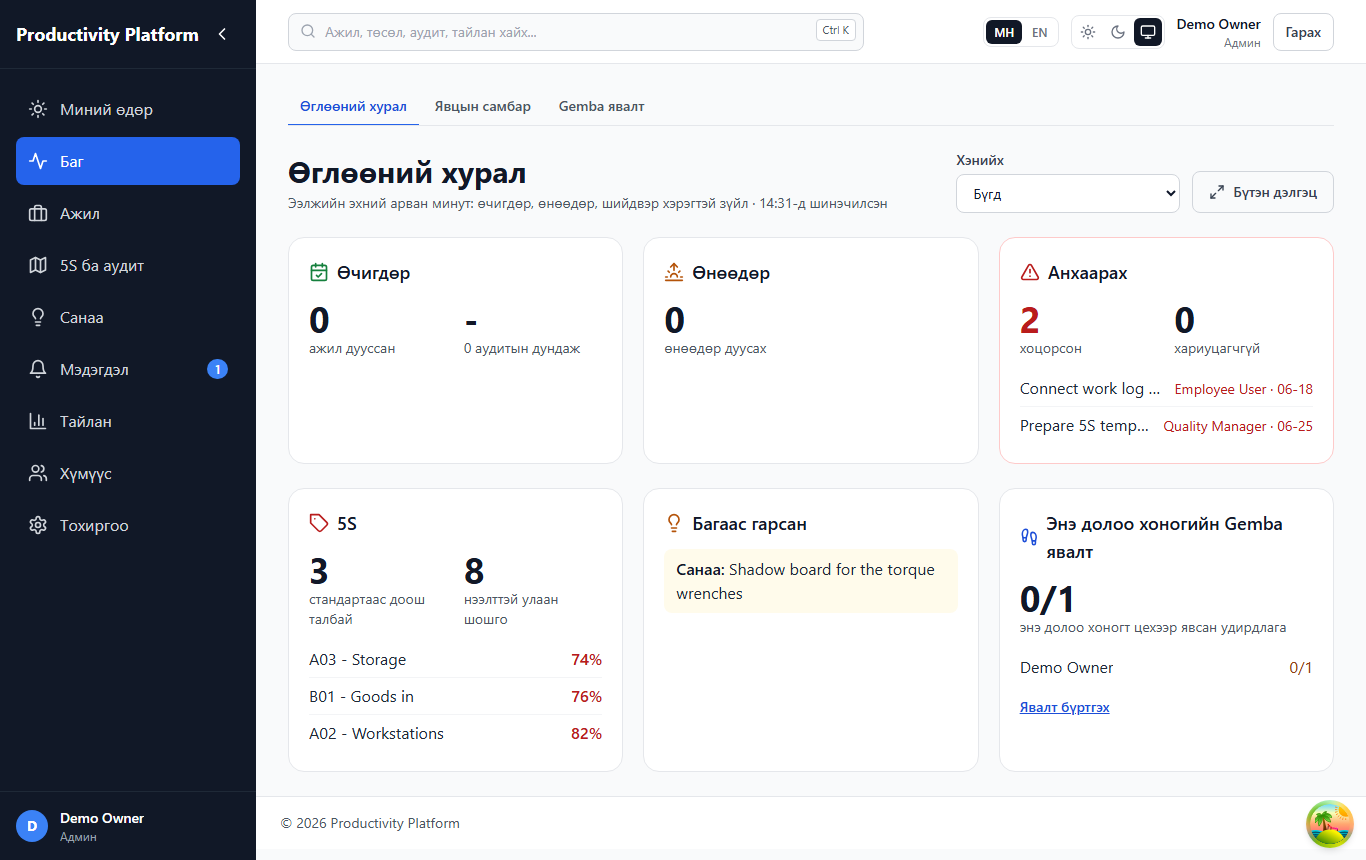
\includegraphics[width=\linewidth]{Figures/ui_huddle.png}
\caption{Өглөөний хурлын самбар}
\label{fig:huddle}
\end{figure}

\begin{figure}[H]
\centering
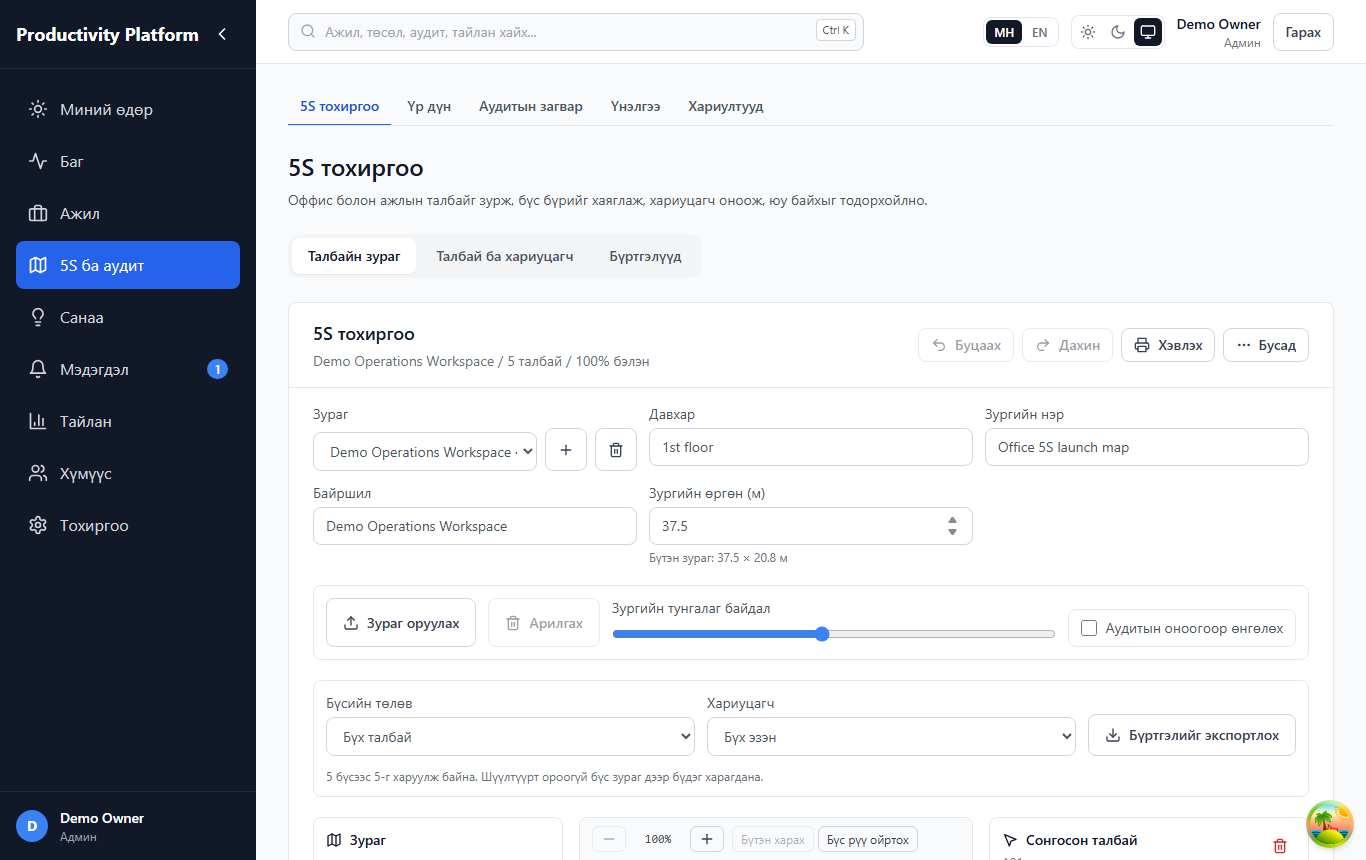
\includegraphics[width=\linewidth]{Figures/ui_fives.png}
\caption{5S талбайн зураг ба бүсийн тохиргоо}
\label{fig:fives}
\end{figure}

Ажилтны нүүр хуудас ``Миний өдөр'' нь тухайн өдрийн ажил, хоцорсон ажил, мэдэгдэл, долоо хоногийн тайлангийн сануулгыг нэг дор харуулна (Зураг~\ref{fig:dashboard}). Ажлын хуудас ажлыг төлөв, хариуцагч, хугацаагаар шүүж харуулна (Зураг~\ref{fig:tasksui}).

\begin{figure}[H]
\centering
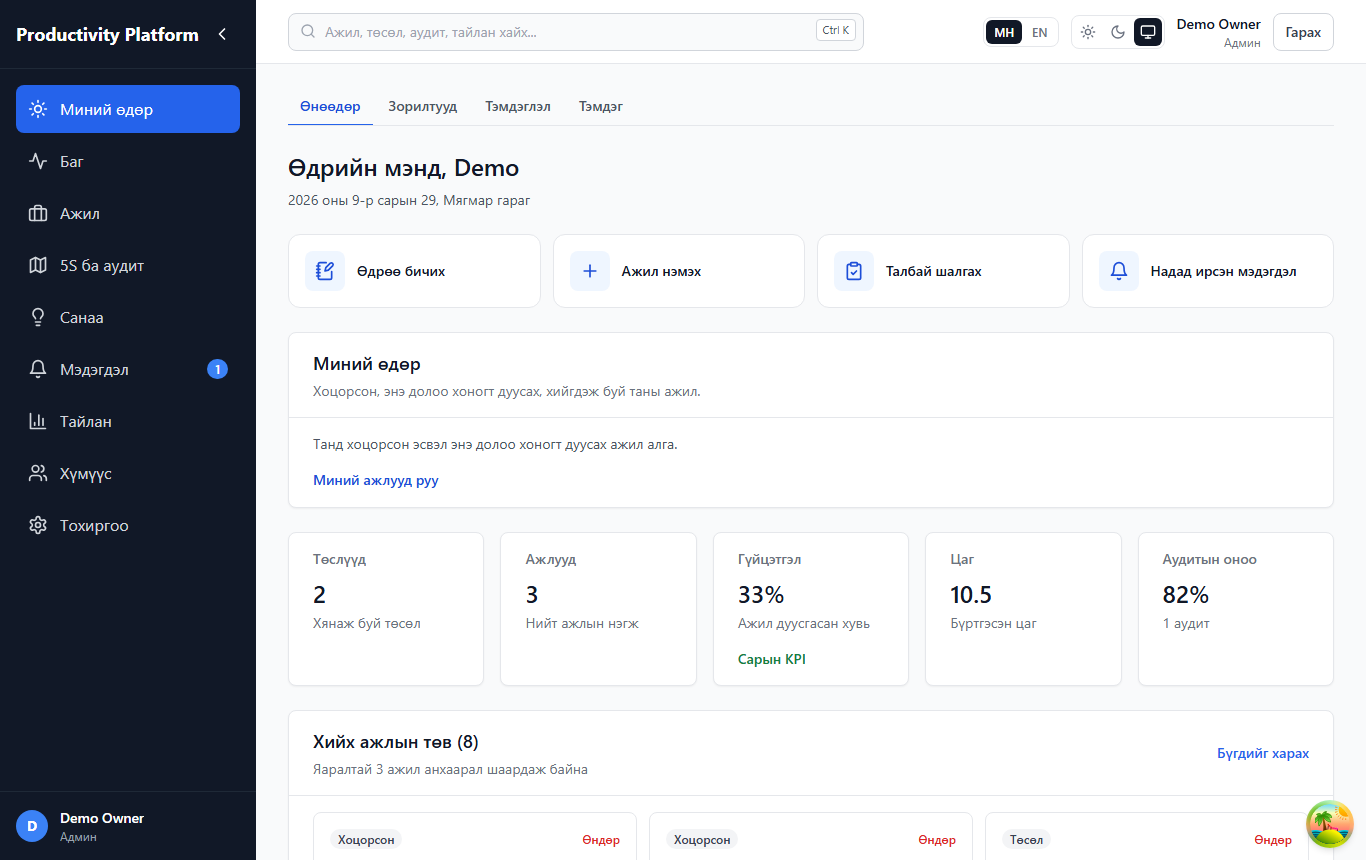
\includegraphics[width=\linewidth]{Figures/ui_dashboard.png}
\caption{``Миний өдөр'' нүүр хуудас}
\label{fig:dashboard}
\end{figure}

\begin{figure}[H]
\centering
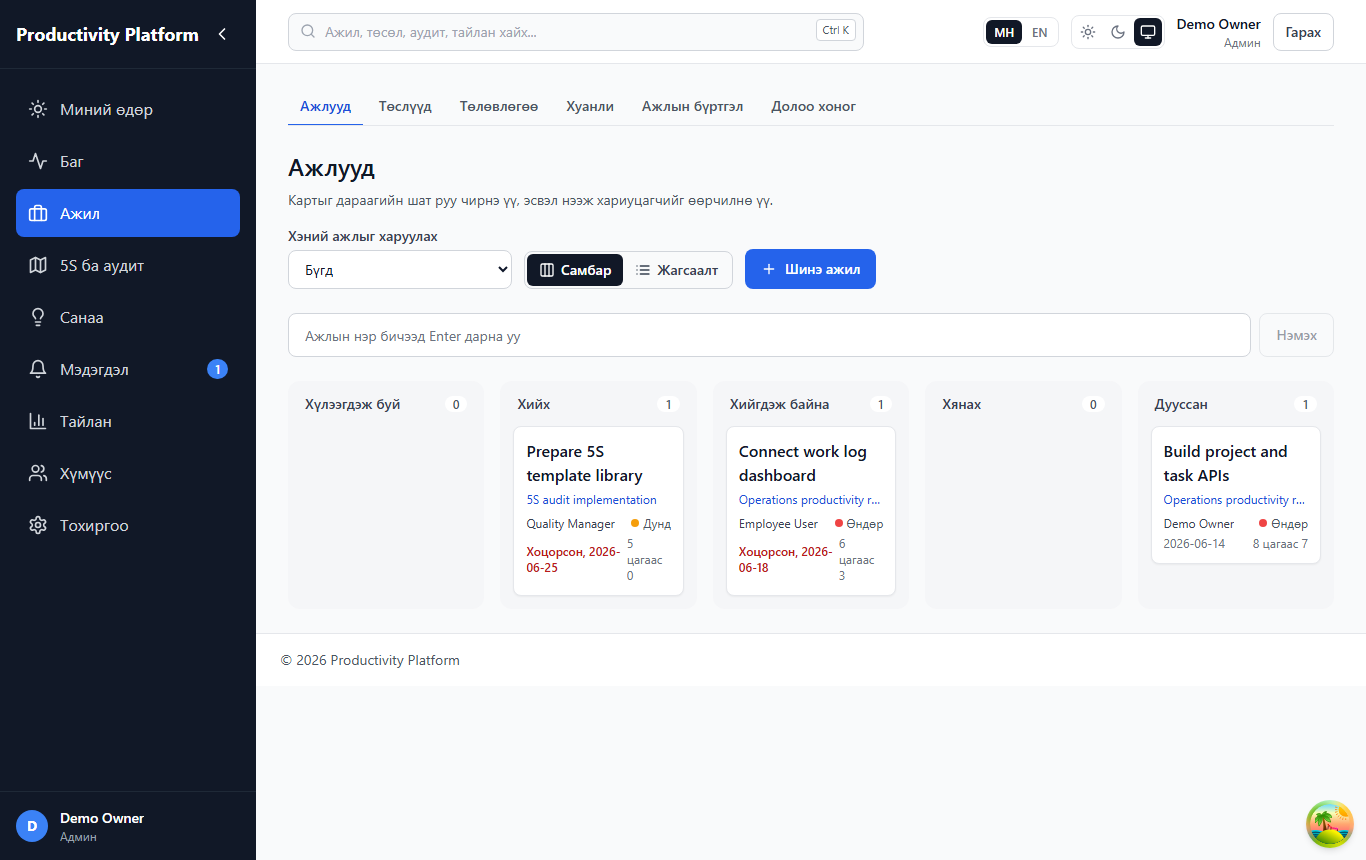
\includegraphics[width=\linewidth]{Figures/ui_tasks.png}
\caption{Ажлын жагсаалт}
\label{fig:tasksui}
\end{figure}

Сарын тайлан бүртгэлээс автоматаар бүрдэх бөгөөд менежер тойм бичвэрийг бичиж эсвэл AI-аар ноороглуулж батална (Зураг~\ref{fig:reportui}). Gemba явалтын хуудсанд менежер ажигласан зүйл, дараагийн алхмуудаа бүртгэж, долоо хоногийн зорилтын биелэлтийг харна (Зураг~\ref{fig:gembaui}).

\begin{figure}[H]
\centering
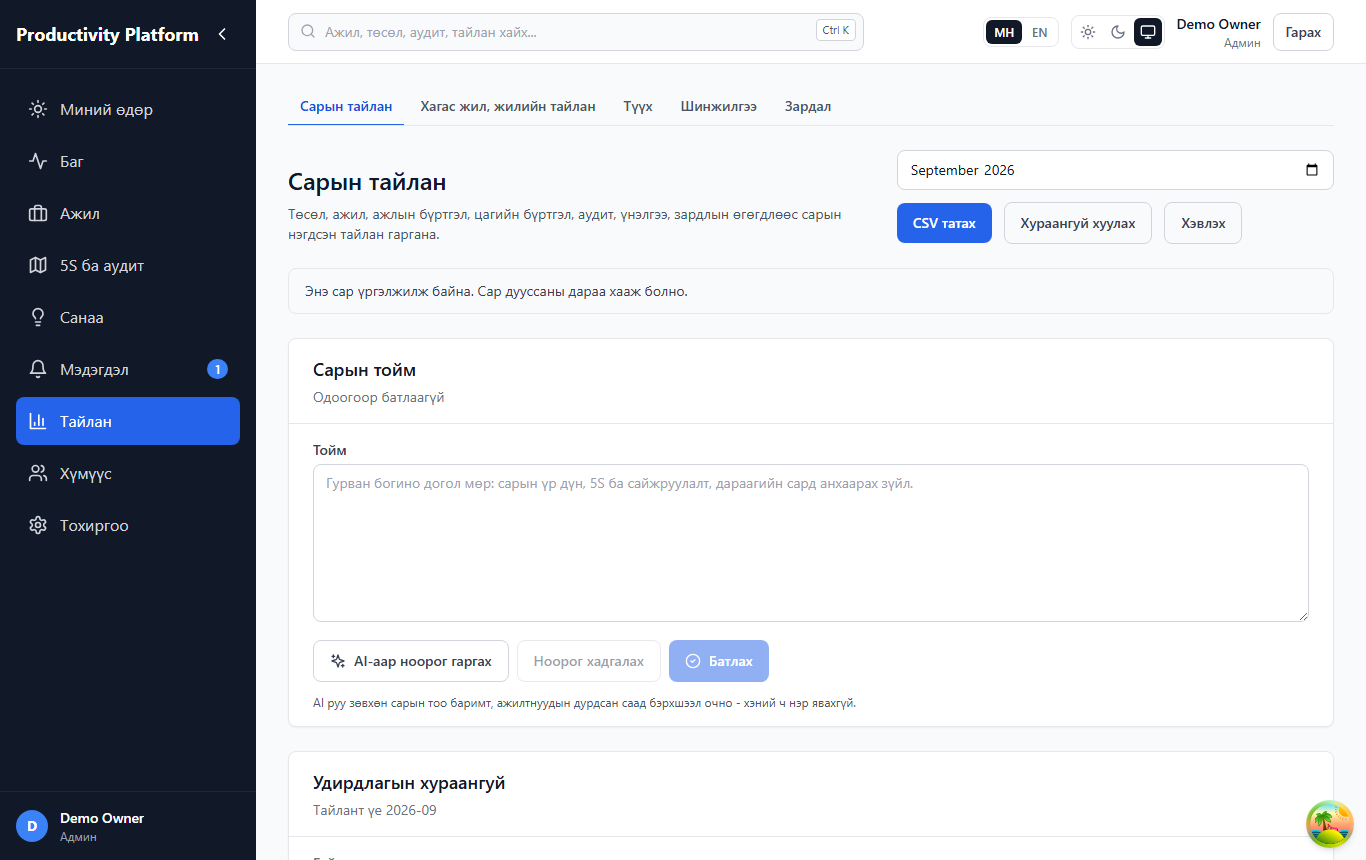
\includegraphics[width=\linewidth]{Figures/ui_report.png}
\caption{Сарын тайлан}
\label{fig:reportui}
\end{figure}

\begin{figure}[H]
\centering
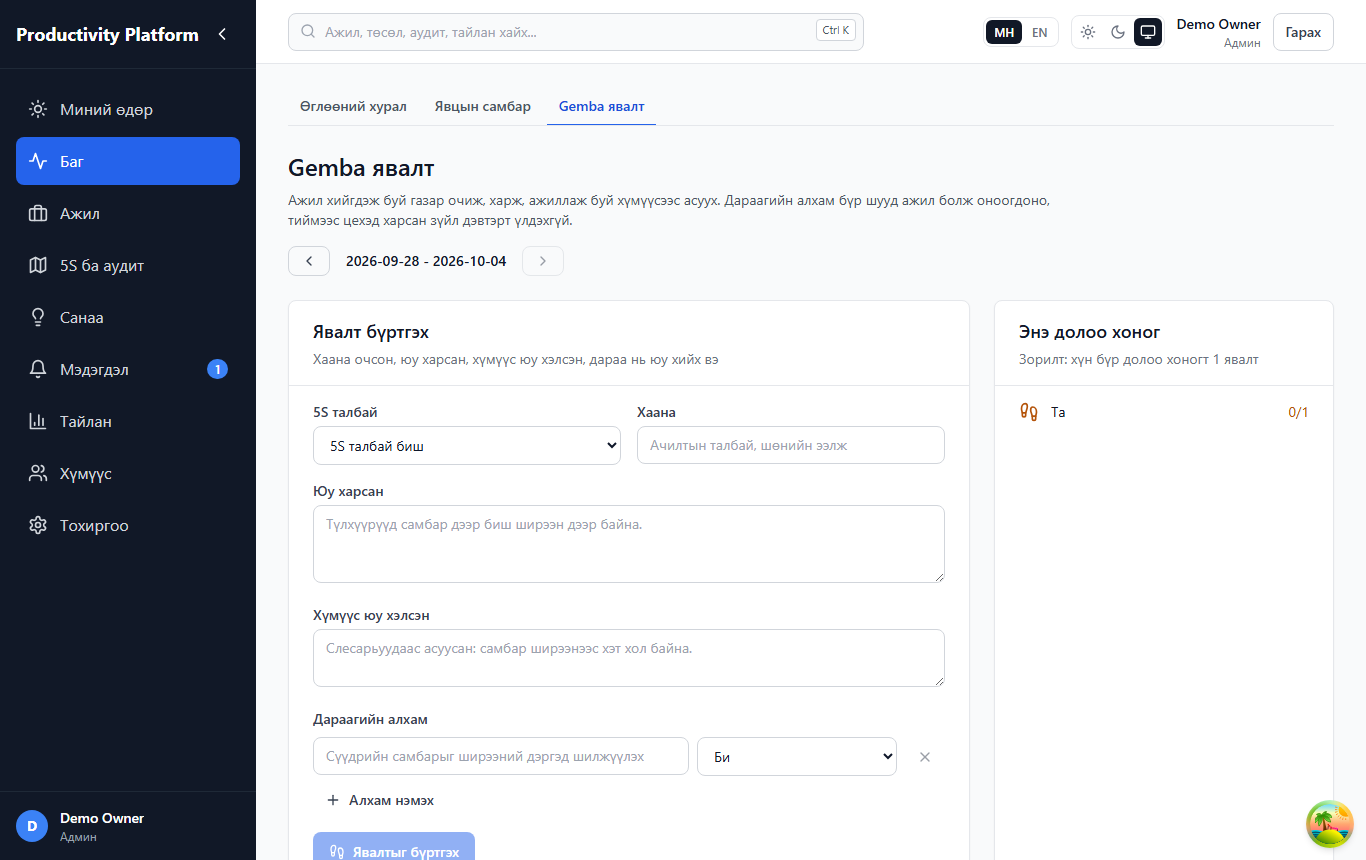
\includegraphics[width=\linewidth]{Figures/ui_gemba.png}
\caption{Gemba явалт бүртгэх}
\label{fig:gembaui}
\end{figure}

Гар утасны апп цех дээрх ажилтанд зориулагдсан. ``Миний ажлууд'' таб ажлыг хоцорсон, өнөөдөр, энэ долоо хоногт гэж бүлэглэж, нэг товшилтоор дуусгах боломж олгоно. 5S табаас талбайг сонгох эсвэл QR шошго уншуулж шалгах хуудсаар аудит хийж, улаан шошго бүртгэнэ. Мэдэгдлийн табаас ирсэн мэдэгдлийг цагтай нь харж, холбогдох таб руу шууд шилжинэ (Зураг~\ref{fig:mobileui}).

\begin{figure}[H]
\centering
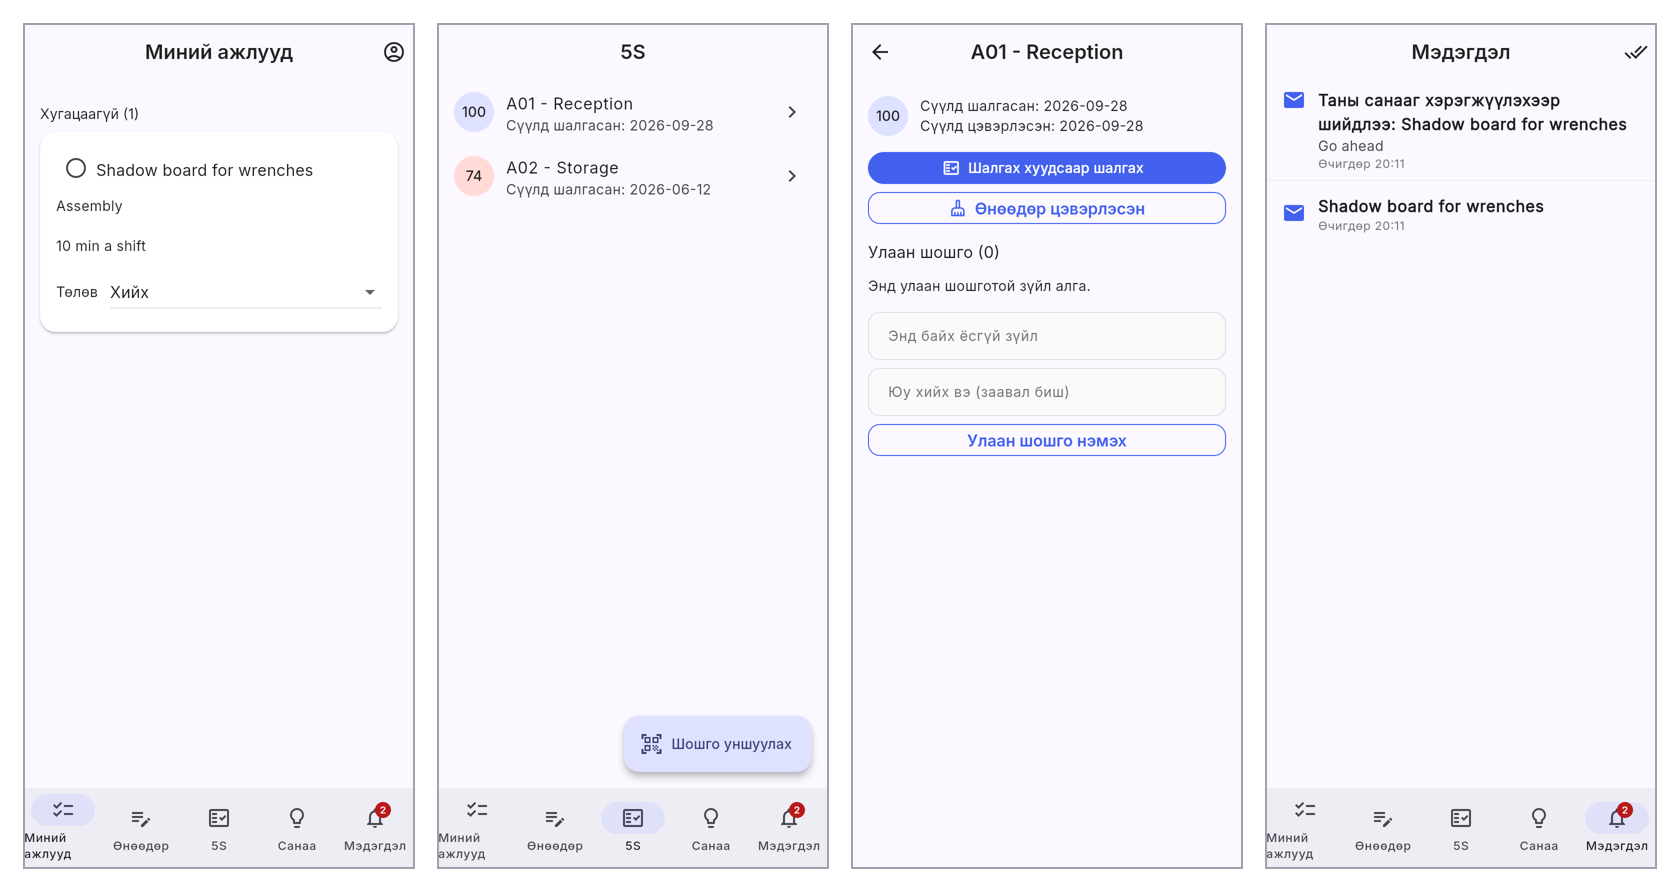
\includegraphics[width=\linewidth]{Figures/ui_mobile.png}
\caption{Гар утасны апп: ажил, 5S талбай, бүс, мэдэгдэл}
\label{fig:mobileui}
\end{figure}

%-------------------------------------------------------------------------------
\section{Системийн туршилтын загвар боловсруулах}
Системийг гурван түвшинд автоматаар туршина (Хүснэгт~\ref{table:tests}). Өөрчлөлт бүрийн дараа бүх тест ажиллаж, амжилтгүй тест байвал өөрчлөлтийг нэгтгэхгүй.

\begin{table}[H]
\centering
\caption{Туршилтын түвшин}
\label{table:tests}
\begin{tabular}{|p{3.2cm}|p{6.4cm}|p{4.6cm}|}
\hline
\textbf{Түвшин} & \textbf{Юуг шалгах} & \textbf{Хэрэгсэл, тоо} \\ \hline
Unit & Оноо тооцох, бүлэглэх, эрх шалгах зэрэг функц & Jest, Vitest, flutter\_test \\ \hline
Integration & API маршрут, өгөгдлийн сан, эрхийн guard & Jest (backend 830 тест) \\ \hline
Component & Вэб хуудас, компонент, орчуулга & Vitest (1017 тест) \\ \hline
End-to-end & Хөтөч дээр бүтэн урсгал, WCAG хүртээмж & Playwright + axe (39 тест) \\ \hline
Гар утас & Дэлгэц, outbox, том үсэг, хүртээмж & flutter\_test (116 тест) \\ \hline
\end{tabular}
\end{table}

Гол туршилтын тохиолдлууд:
\begin{enumerate}[label=(\alph*)]
    \item Нэвтрэх -- зөв, буруу нууц үг, идэвхгүй бүртгэл.
    \item 5S аудит -- оноо 85\%-иас доош бол засах ажил нэг удаа үүсэх; дахин илгээхэд давхардахгүй.
    \item Сүлжээгүй горим -- сүлжээгүй үед хадгалагдаж, сүлжээ сэргэхэд илгээгдэх; 4xx хариуг дахин илгээхгүй.
    \item Эрх -- ажиглагч ажил устгах хүсэлт илгээхэд 403 буцах.
    \item Сарын тайлан -- хаагдсан сарын тайлан дараа нь өгөгдөл өөрчлөгдсөн ч хэвээр байх.
\end{enumerate}

\section*{Бүлгийн дүгнэлт}
Энэ бүлэгт системийн давхаргат архитектур, зохиомжийн класс, дарааллын диаграмм, өгөгдлийн сангийн схем, эрхийн загварыг боловсруулав. Аудитын оноо ба засах ажил, сүлжээгүй горимын дараалал, өдрийн сануулга, сарын тайлан, бүтээмжийн үзүүлэлт, ажлын бүлэглэлт гэсэн зургаан алгоритмыг зохиомжилж, байршуулалтын диаграмм болон туршилтын загварыг тодорхойлов.
